\documentclass[12]{article}
\usepackage[spanish,english]{babel}
%\usepackage[spanish]{babel}
\usepackage[utf8]{inputenc}
\usepackage{graphicx}
\usepackage{epsfig}
\usepackage{multirow}
\usepackage{multicol,caption}
\usepackage{amsthm} % Theorem Formatting
\usepackage{amssymb}    % Math symbols such as \mathbb
\usepackage{color}
\usepackage{hyperref}
\usepackage[none]{hyphenat}
\usepackage{appendix}
\usepackage{pdfpages}
\renewcommand{\appendixname}{Anexo}
\renewcommand{\appendixtocname}{LISTA DE ANEXOS}
\renewcommand{\appendixpagename}{Anexos}
%\renewcommand{\tablename}{Tabla}
%\def\tablename{Cuadro}% por \def\tablename{Tabla}% 
\newenvironment{Figure}
{\par\medskip\noindent\minipage{\linewidth}}
{\endminipage\par\medskip}
\addto\captionsspanish{%
\def\tablename{Tabla}%
}
\topmargin  = 10pt
\oddsidemargin  = -0.5in
%\headheight = 12pt
%\headsep    = 15pt
%\footskip   = 15pt
\textheight = 21.5 cm
\textwidth  = 18.5cm
\tolerance=10000
\title{\bf{Modulo motorizado para ilustrar la difracción, atenuación y absorción de ondas electromagnéticas en el espectro infrarrojo; utilizando tecnologías libres y de bajo costo.}}
\author{Diego Parra\footnote{diegoestudianteud1@gmail.com}, Julian Salamanca\footnote{jasalamanca@udistrital.edu.co} \\
  Universidad Distrital, Calle 3 No 26A-40 Bogotá-Colombia\\
  Grupo de Física e Informática ``FISINFOR''
}
\date{\today}
\begin{document}
%\def\tablename{Cuadro}% por \def \tablename{Tabla}% 
\renewcommand{\tablename}{Tabla}
\maketitle
\vspace{-0.8cm}
\selectlanguage{english}
\begin{abstract}

This writing describes in detail the construction of a motor vehicle taking advantage of the technological wonders of semiconductors to control hardware with a ATMEGA328P-PU microcontroller with serial communication via Bluetooth to a computer whose operating system is GNU-Linux, equipped with a side infrared sensor illustrating the diffraction phenomenon and calculates the wavelength emitted by the lED diode emitting infrared; also it has a pair of emitter sensors - infrared receiver on the front of the vehicle, the infrared sensor front and infrared emitter front illustrate the law of decay density radiansa with the square of the distance to the radiating source, the reflectance and transmittance that occurs due to the interaction of the radiation with matter. \\\\
This project also has instructions for using the control software free infrarossi and their respective installation, whose function is to control the actions taken by the infrarossi vehicle, both forward and capture data from the side and front sensors and control the radiant source photon in the infrared, for examination. It is noteworthy that all this communication between the motor module infrarossi and control software comes pre designed to be via bluetooth.
{\bf{Keywords:}} infrarossi motorized module,  control software free infrarossi, law decay density radiansa with the inverse square, reflectance, diffraction, serial communication, bluetooth, GNU-Linux, software, hardware.
\selectlanguage{spanish}
\begin{center}
{\bf{Resumen}} 
\end{center}
  
El presente escrito, describe detalladamente la construcción de un vehículo motorizado  aprovechando las maravillas tecnológicas de los semiconductores para el control de hardware con un microcontrolador atmega328P-PU, con comunicación serial vía bluetooth con un ordenador cuyo sistema operativo es GNU-Linux, equipado con un sensor  infrarrojo lateral que ilustra el fenómeno de difracción y calcula la longitud de onda emitida por el diodo led emisor en infrarrojo; también tiene un par de sensores emisor – receptor infrarrojo en la parte del frente del vehículo, el sensor infrarrojo frontal y el emisor infrarrojo frontal ilustran la ley del decaimiento de  la densidad de radiansa con el cuadrado de la distancia a la fuente radiante,  la reflectancia y  transmitancia que ocurre debido a la interacción de esta radiación con la materia.\\\\
Este proyecto cuenta también con las indicaciones para el uso del software de control free infrarossi y su respectiva instalación, cuya función es controlar las acciones que realiza el vehículo infrarossi, tanto  avanzar  y capturar datos de los sensores  lateral y frontal como de controlar la fuente radiante de fotones en el infrarrojo, para su respectivo análisis. Cabe mencionar que toda esta comunicación entre el modulo motorizado infrarossi y su software de control viene pre diseñada para que sea  vía bluetooth.
\\
{\bf{Descriptores:}}Modulo motorizado infrarossi, software de control free infrarossi, ley de decaimiento de la densidad de radiansa con el inverso del cuadrado, reflectancia, difracción, comunicación serial, bluetooth GNU-Linux, software, hardware.
\end{abstract}
%tabla de contenido sin numeracion
%\renewcommand\contentsname{\centering TABLA DE CONTENIDO}
%\thispagestyle{empty}
%\setcounter{page}{1}
%\tableofcontents
%\clearpage
%lista de figuras
%\renewcommand\listfigurename{\centering LISTA DE FIGURAS}
%\listoffigures
%\clearpage
%lista de tablas
% \renewcommand\listtablename{\centering LISTA DE TABLAS}
% \listoftables
% \clearpage
\begin{multicols}{2}
\section{Introducción}
\selectlanguage{spanish}
En la actualidad, una cantidad de instrumentos de laboratorio para la enseñanza en física y especialmente de  fenómenos electromagnéticos,  transporte e inyección de energía a los portadores de carga en los semiconductores, fenómenos ondulatorios, etc.; son  muy costosos, incluso estos instrumentos son exclusivos de los departamentos de ciencias en diferentes  universidades y laboratorios, lo que dificulta el contacto de la población a estas manifestaciones físicas; un caso especial es el estudio de las propiedades de las ondas electromagnéticas y su dualidad onda – partícula, en determinadas frecuencias “caso clásico” o en paquetes de energía discreta según su longitud de onda “caso cuántico”; específicamente en cuestión de frecuencias o longitudes de onda que corresponden al espectro electromagnético infrarrojo, concretamente cuando se habla de difracción, atenuación, absorbancia, transmitancia, reflectancia,   ley de decaimiento de la densidad de radiansa con el inverso del cuadrado de la distancia a la fuente; solo se tiene como marco de estudio de estos fenómenos fenómenos ondulatorios infrarrojos a la espectrometría  infrarroja, que es usada habitualmente por estudiantes de medicina, química, biología, etc., muy especializados, con instrumentos muy costosos y precisos;  lo que deja sin aproximarse a los demás estudiantes de ciencias exactas a estos tópicos de la física que están presentes en la vida diaria y que no son visibles al ojo humano.\\\\
El objetivo de este trabajo de grado es diseñar un instrumento de laboratorio que sea capaz de ilustrar tres  fenómenos físicos  de la radiación electromagnética y su dualidad onda – partícula; los cuales son: difracción en infrarrojo, reflectancia en el infrarrojo y ley del decaimiento de la irradiansa con el inverso del cuadrado de la distancia a la fuente. Esto con el fin de dejar  referencia que en la actualidad no se estudia de manera cómoda los fenómenos ondulatorios y de interacción de esta manifestación física de la energía con la materia, en el espectro de está longitud de onda como lo es el infrarrojo. \\\\
Por esta razón se elabora muy cuidadosamente un instrumento que llene las expectativas de aprendices y docentes de carreras afines a  estos asuntos;  el cual es económico, con materiales de fácil acceso, que es capaz de aproximar al educando a fenómenos como lo es la difracción, la ley del decaimiento de  la densidad de radiansa con el inverso del cuadrado de la distancia a la fuente radiante,  la reflectancia y  transmitancia que ocurre debido a la interacción de esta radiación con la materia, en el rango infrarrojo del espectro.  \\\\
A este instrumento se le denomino $modulo$ $motorizado$ $infrarossi$, el cual es un vehículo de tracción electromagnética, con comunicación serial vía bluetooth con un ordenador GNU-Linux, equipado con un sensor infrarrojo lateral para ilustrar el fenómeno de difracción, un sensor infrarrojo frontal y un emisor infrarrojo frontal para ilustrar la ley del decaimiento de  la densidad de radiansa con el cuadrado de la distancia a la fuente radiante,  la reflectancia y  transmitancia que ocurre debido a la interacción de esta radiación con la materia; el modulo infrarossi es capaz de acercar de manera cualitativa y cuantitativa al estudio de estos contenidos, pues aparte del instrumento que obtiene los datos, también cuenta con un software de control   y análisis de datos obtenidos, a este software se le designo el nombre de $software$ $de$ $control$ $free$ $infrarossi$, el cual complementa el modulo motorizado infrarossi, convirtiéndolo en una herramienta de laboratorio muy precisa, económica, fácil de utilizar, con su propio repositorio en github, con buena  documentación, fácil de manipular e instalar.
\section{Diseño experimental}
El modulo motorizado infrarossi ver figuras \ref{fig:Mon_meca} , \ref{fig:Mon_chasis_supe} , \ref{fig:Mon_meca_sup} y \ref{fig:Mon_vis_inf}, en el anexo B; es un vehículo con chasis de madera,  batería de $9 V$ del tipo cuadrada recargable,  modulador de señal de $9 V$ a  $5 V$ voltaje continuo, tracción electromagnética con  transmisión de tipo engranaje trasera con diferencial cero de eje posterior fijo y eje delantero fijo, cuatro llantas de cinco centímetros de diámetro y dos centímetros de ancho, comunicación bluetooth entre vehículo y ordenador, dos  sensores de intensidad lumínica en el rango infrarrojo del espectro electromagnético de estructura epoxy cinco milímetros, uno del tipo radar sin barrido basado en el principio de electro-recepción\cite{ELECTRORRECPCION} activa con disposición espacial en la parte media del sector frontal,  y en la zona lateral derecha a siete centímetros del sector frontal reposa el sensor del tipo radar sin barrido basado en el principio de electro-recepción pasiva, control de rapidez en el avance del vehículo y control de hardware del vehículo. 
%---------------------Disposición electrica 
\subsection{Disposición eléctrica}
El modulo infrarossi es un vehículo didáctico para la enseñanza experimental en física ver figuras \ref{fig:cir_proto_elec} y \ref{fig:cir_elec} , los diferentes sistemas electrónicos del vehículo pueden removerse en cuatro sistemas: control de hardware y comunicación bluetooth con ordenador ver figura \ref{fig:control_hardware}, control rapidez del vehículo ver figura \ref{fig:control_avance}  , sensor electro-recepción pasiva ver figura \ref{fig:recepcion-pasiva} , y, un sensor de electro-recepción activa ver figura \ref{fig:recepcion-activa} . 
%------------------------control de hardware.....
\subsubsection{Control de hardware}
El modulo infrarossi tiene un sistema de control de hardware ver figura \ref{fig:control_hardware}, que le indica al vehículo cuando debe avanzar, cuando debe detenerse, la rapidez con que debe avanzar, la distancia que debe avanzar, activar y detener el sensor de electro-recepción pasiva y enviar los datos vía bluetooth al ordenador, activar y detener el sensor de electro-recepción activa y enviar los datos vía bluetooth al ordenador, enviar señales del proceso que esta realizando con el encendido y apagado de diodos leds de colores y mantener una comunicación continua con el ordenador vía bluetooth.   \\ \\
%-------------------------------------Sistema  tarjeta, oscilador para atmega 
\begin{Figure}
\center
\begin{tabular}{|l|r|}
\hline
\\
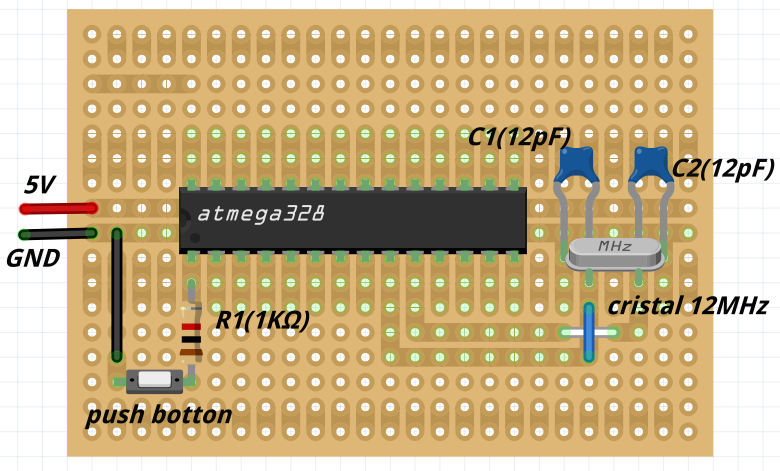
\includegraphics[width=8cm, height=5cm]{img/F1.png}  \\\\ \hline
\end{tabular}
\captionof{figure}{Esquema tarjeta perforada con microcontrolador atmetga 328, cristal oscilador $12 MHz$, dos condensadores cerámicos de $12 pF$, resistencia de $1k\Omega$ y un botón; los cables de color negro son tierra, los de color rojo son voltaje, el cable azul y blanco son puentes. Figura generada en Fritzing.}
\label{fig:Mon_micro}
\end{Figure}
El control de hardware ver figura \ref{fig:Esq_elec_final_con_har} , está basado en un microcontrolador atmega\cite{ARDUINO} 328P-PU de 28 pines, con un voltaje de operación de $5 V$, una corriente máxima de  $40 mA$ por pin de salida, la suma de corriente en todas las salidas del microcontrolador no excede los  $150 mA$, trabaja en una frecuencia de 12 MHz. Este dispositivo consta de un modulador de frecuencia, un modulador de señal de $9V$ a $5V$ voltaje continuo, un modulo de comunicación tipo bluetooth, un botón de reinicio y un led indicador de procesos. \\ \\
El modulador de frecuencia como se muestra en las figuras \ref{fig:Mon_micro} y \ref{fig:Esq_micro} , sincroniza el reloj interno del microcontrolador, calibrando los tiempos en los procesos del microcontrolador con los indicados por el fabricante y que reposan en la pagina oficial del proyecto arduino\footnote{Pagina oficial proyecto arduino, [on line] https://www.arduino.cc/} .

%-------------------------------------esquema electrico, oscilador para atmega 
\begin{Figure}
\center
\begin{tabular}{|l|r|}
\hline
\\
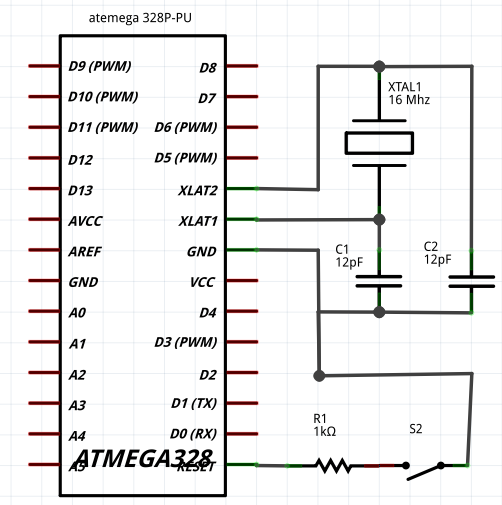
\includegraphics[width=8cm, height=5cm]{img/G1.png}  \\\\ \hline
\end{tabular}
\captionof{figure}{Esquema eléctrico microcontrolador atmetga 328, cristal oscilador $12 MHz$, dos condensadores cerámicos de $12 pF$, resistencia de $1k\Omega$ y un botón. Figura generada en Fritzing.}
\label{fig:Esq_micro}
\end{Figure}
El botón de reinicio o switch de reset como se muestra en las figuras \ref{fig:Mon_micro} y \ref{fig:Esq_micro}, este interruptor reinicia el firmware cargado dentro del microcontrolador cuando surge algún conflicto interno en los procesos de este dispositivo. 
%-------------------------Modulador de voltaje
\begin{Figure}
\center
\begin{tabular}{|l|r|}
\hline
\\
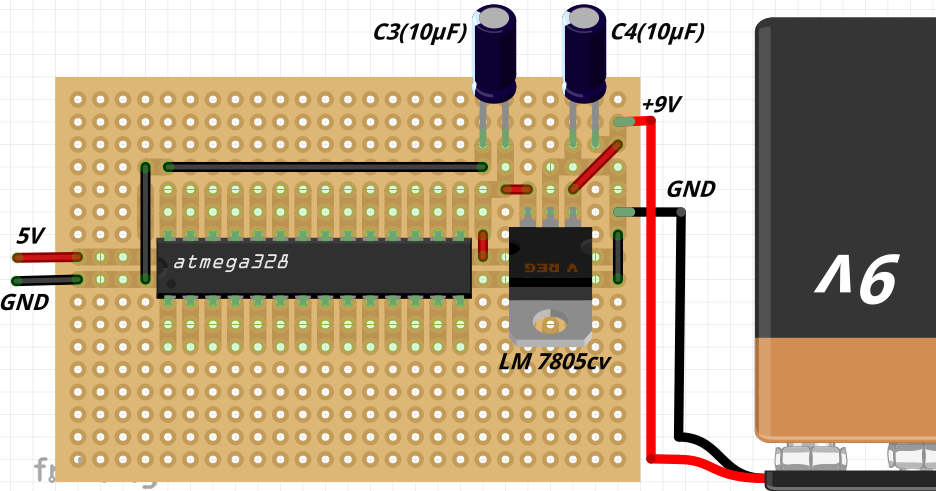
\includegraphics[width=8cm, height=5cm]{img/F2.png}  \\\\ \hline
\end{tabular}
\captionof{figure}{Esquema tarjeta perforada microcontrolador atmetga 328, transistor LM 7805 cv, dos condensadores electroliticos de $10 \mu F$, conectados a batería de $9 V$. Figura generada en Fritzing.}
\label{fig:Mon_regula}
\end{Figure}
\vspace{1cm}
El modulador de señal como se muestra en las figuras \ref{fig:Mon_regula} y \ref{fig:Esq_regula} , filtra la señal de entrada de $9 V$ voltaje continuo a la señal de trabajo óptima del microcontrolador y los diferentes sistemas electrónicos cual es de $5 V$ voltaje continuo. 
%-------------------------------------Esquema electrico modulador de voltaje
\begin{Figure}
\center
\begin{tabular}{|l|r|}
\hline
\\
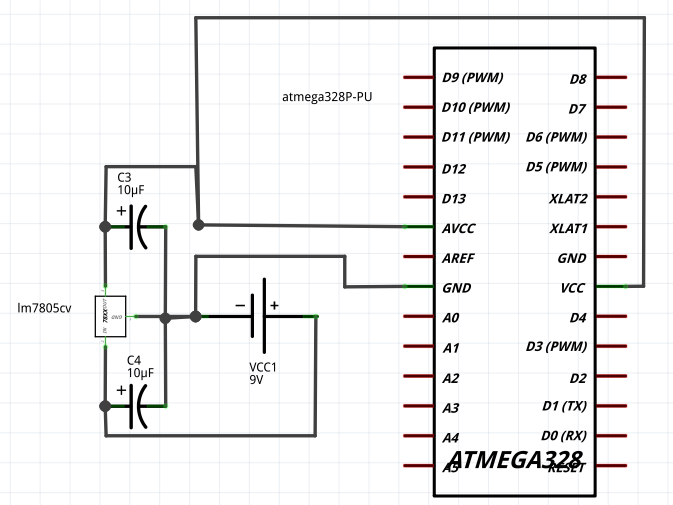
\includegraphics[width=8cm, height=5cm]{img/G2.png}  \\\\ \hline
\end{tabular}
\captionof{figure}{Esquema eléctrico microcontrolador atmetga 328, transistor LM 7805 cv, dos condensadores electroliticos de $10 \mu F$, conectados a batería de $9 V$. Figura generada en Fritzing.}
\label{fig:Esq_regula}
\end{Figure}
La comunicación del microcontrolador con el ordenador como se muestra en las figuras  \ref{fig:Mon_blue} y \ref{fig:Esq_blue} la ejecuta el modulo bluetooth hc-05; de esta manera el software de control free infrarossi tiene completo dominio del hardware del vehículo motorizado infrarossi.
%-----------------------------Sistema bluetooth
\begin{Figure}
\center
\begin{tabular}{|l|r|}
\hline
\\
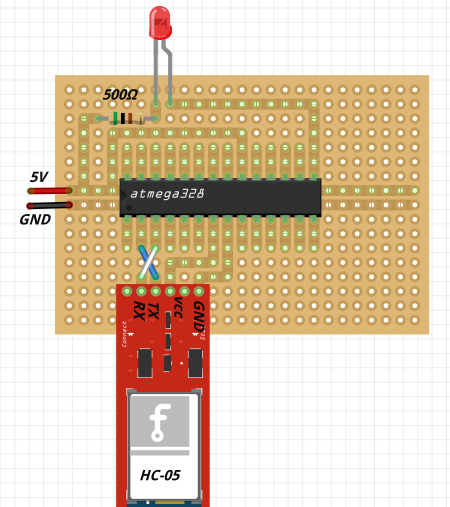
\includegraphics[width=7cm, height=5cm]{img/F3.png}  \\\\ \hline
\end{tabular}
\captionof{figure}{Esquema tarjeta perforada microcontrolador atmetga 328, modulo bluetooth hc-05, diodo led de 3mm y una resistencia de $500 \Omega$. Figura generada en Fritzing.}
\label{fig:Mon_blue}
\end{Figure}
El avance espacial del vehículo como el encendido y apagado de los diferentes sensores del dispositivo, junto con la recolección de datos de los sensores y la verificación del proceso que realiza la tarjeta, son enviados por el modulo $hc -05$ al ordenador, para su respectivo análisis; de igual forma las ordenes provenientes del software de control via bluetooth son recibidas por el modulo $hc-05$ y enviadas al microcontrolador para su inmediata ejecución. \\
%------------------------------Esquema electrico sistema bluetooth
\begin{Figure}
\center
\begin{tabular}{|l|r|}
\hline
\\
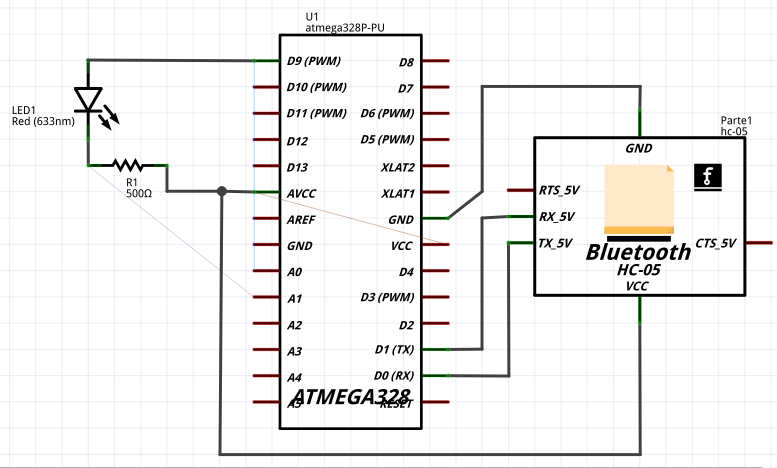
\includegraphics[width=8cm, height=5cm]{img/G3.png}  \\\\ \hline
\end{tabular}
\captionof{figure}{Esquema eléctrico microcontrolador atmetga 328, modulo bluetooth hc-05, diodo led de 3mm y una resistencia de $500 \Omega$. Figura generada en Fritzing.}
\label{fig:Esq_blue}
\end{Figure}
El diodo led que se observa en las figuras  \ref{fig:Mon_blue} y \ref{fig:Esq_blue} es un indicador lumínico de los procesos que esta realizando el microcontrolador. 
%------------------------------MONTAJE FINAL
\begin{Figure}
\center
\begin{tabular}{|l|r|}
\hline
\\
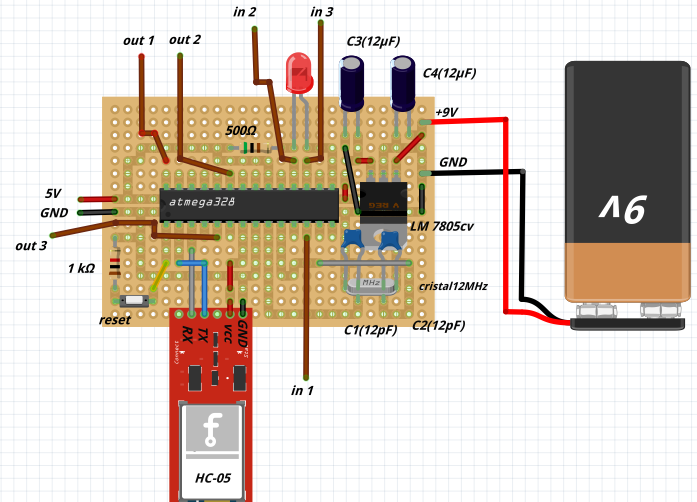
\includegraphics[width=8cm, height=6cm]{img/F6.png}  \\\\ \hline
\end{tabular}
\captionof{figure}{Esquema en tarjeta perforada del microcontrolador atmetga 328, con las disposiciones del sistema de control de hardware. Figura generada en Fritzing.}
\label{fig:Esq_elec_final_con_har}
\end{Figure}
\vspace{1cm}
El control de hardware que se observa en las figuras \ref{fig:Esq_elec_final_con_har}, \ref{fig:Esq_elec_final_} y \ref{fig:Esq_PCB_final}, consta de un modulador de señal LM 7805cv, modulador de frecuencia con oscilador 12 Mhz, el pin IN2 es la conexión a led de color 3mm,  el pin IN3 es la conexión a led de color 3mm, pin de salida a +5v, pin de salida a GND, modulo bluetooth hc-05, botón de reinicio, microcontrolador atmega 328P-PU, el pin OUT1 es la salida al sensor de electro-recepción activa, el pin OUT2 es la salida al sensor de electro-recepción pasiva, el pin OUT3 es el pin de salida al sistema de control de velocidad, el pin IN1 es la salida al diodo emisor infrarrojo; la placa perforada tiene dimensiones de  $6x4.5 cm^{2}$ , con un acabado en velcro, lo que facilita el montaje de la misma en el vehiculo.
%------------------------------esquema electrico MONTAJE FINAL
\begin{Figure}
\center
\begin{tabular}{|l|r|}
\hline
\\
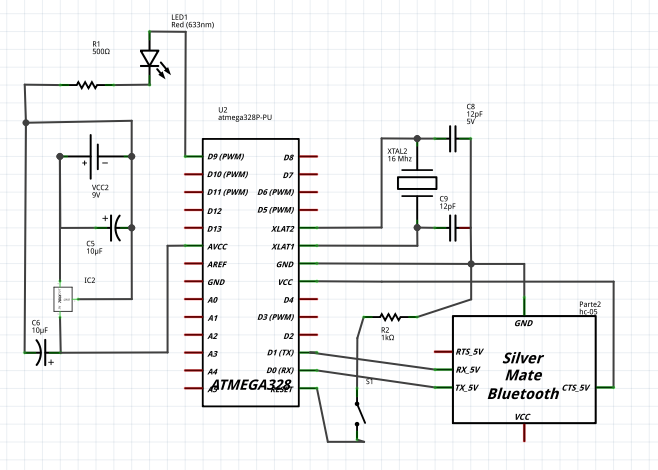
\includegraphics[width=8cm, height=6cm]{img/G4.png}  \\\\ \hline
\end{tabular}
\captionof{figure}{Esquema eléctrico microcontrolador atmetga 328, con las disposiciones del sistema de control de hardware. Figura generada en Fritzing.}
\label{fig:Esq_elec_final_}
\end{Figure}
\subsubsection{Control de avance}
El sistema de control de avance ver figura \ref{fig:control_avance}  , es el que da el movimiento del vehículo únicamente hacia adelante, pues no consta de un sistema de reversa, esta peculiaridad del vehículo permite que este avance una cantidad mínima de distancia para la recolección de datos de los distintos sensores de electro-recepción que dispone el vehículo. \\ \\
El sistema de control en el avance del vehículo infrarossi como se observa en las figuras \ref{fig:perfo_sis_con} , \ref{fig:cirele_sis_con} y \ref{fig:PCB_sis_con} , consta de dos salidas a GND, dos salidas a +5V, una entrada a GND, una entrada a +5V, un tip 122, una resistencia de $5k\Omega$, diodo 1N4001, el pin OUT3 es la salida al pin D3(PWM) del microcontrolador atmega, salida M1 para el motor, salida M2 para el motor; un motor de corriente directa de medio vatio de potencia con sistema de transmisión de engranaje de eje fijo como se observa en la figura \ref{fig:Mon_vis_inf}.\\\\
El pin D3(PWM) del microcontrolador envía una señal de $24mA$ al pin base del tip\cite{TIP122} 122, durante 37 ms, dando un avance de 2mm al vehículo motorizado infrarossi.
%------------------------------circuito impreso MONTAJE FINAL
\begin{Figure}
\center
\begin{tabular}{|l|r|}
\hline
\\
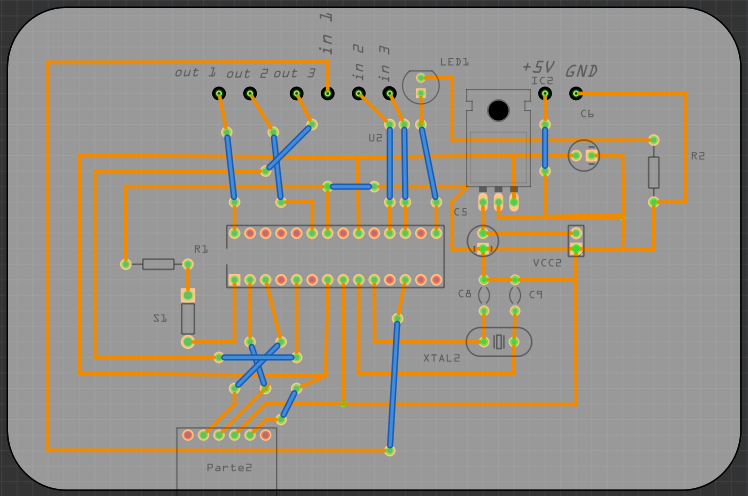
\includegraphics[width=8cm, height=6cm]{img/H3.png}  \\\\ \hline
\end{tabular}
\captionof{figure}{Esquema de tarjeta impresa para el microcontrolador atmetga 328P-PU,  con las disposiciones del sistema de control de hardware. Figura generada en Fritzing.}
\label{fig:Esq_PCB_final}
\end{Figure}


%------------------------Sistema control avance tarjeta perforada
\begin{Figure}
\center
\begin{tabular}{|l|r|}
\hline
\\
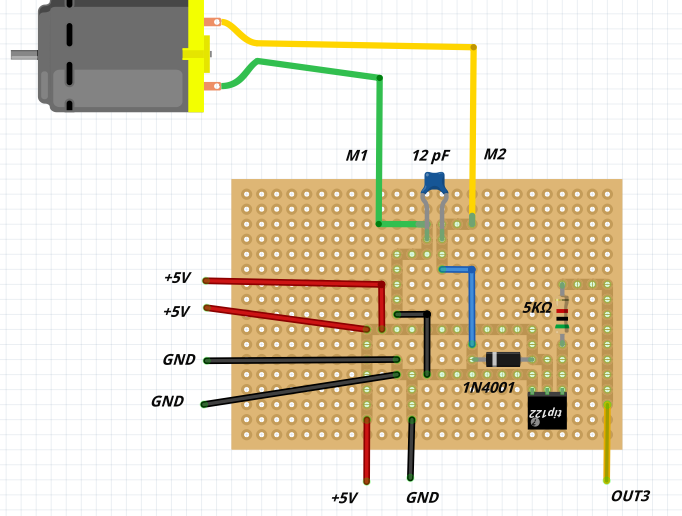
\includegraphics[width=8cm, height=6cm]{img/F8.png}  \\\\ \hline
\end{tabular}
\captionof{figure}{Esquema tarjeta perforada del sistema de control de avance. Figura generada en Fritzing.}
\label{fig:perfo_sis_con}
\end{Figure}

%------------------------Sistema control avance montaje protoboard
%\begin{Figure}
%\center
%\begin{tabular}{|l|r|}
%\hline
%\\
%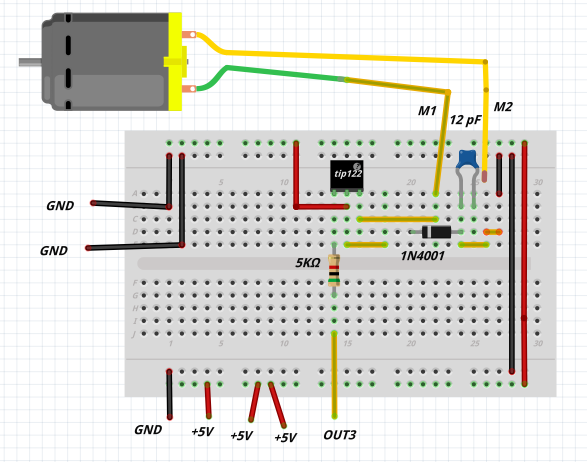
\includegraphics[width=8cm, height=5cm]{img/F7.png}  \\\\ \hline
%\end{tabular}
%\captionof{figure}{Esquema en protoboard del sistema de control de avance. Figura generada en Fritzing.}
%\label{fig:proto_sis_con}
%\end{Figure}
%------------------------Sistema control avance circuito eléctrico
\begin{Figure}
\center
\begin{tabular}{|l|r|}
\hline
\\
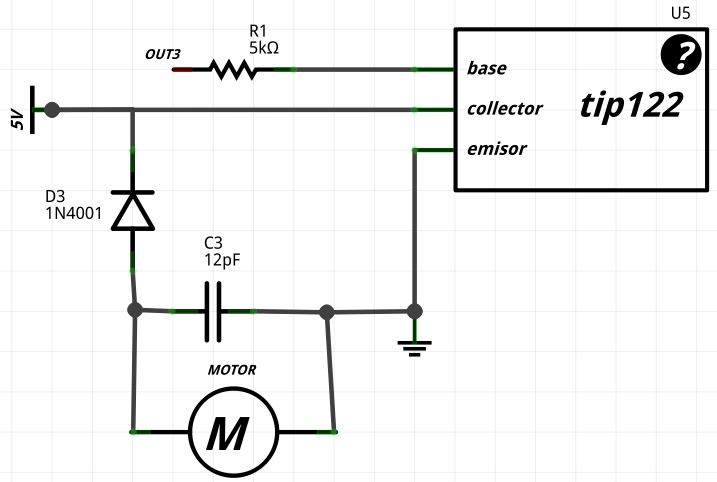
\includegraphics[width=8cm, height=5cm]{img/tip122.png}  \\\\ \hline
\end{tabular}
\captionof{figure}{Esquema del circuito eléctrico del sistema de control de avance. Figura generada en Fritzing.}
\label{fig:cirele_sis_con}
\end{Figure}
%------------------------Sistema control avance tarjeta de circuito impreso
\begin{Figure}
\center
\begin{tabular}{|l|r|}
\hline
\\
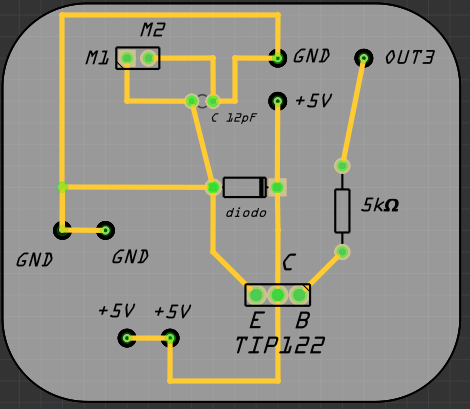
\includegraphics[width=8cm, height=5cm]{img/H4.png}  \\\\ \hline
\end{tabular}
\captionof{figure}{Tarjeta de circuito impreso el sistema de control de avance. Figura generada en Fritzing.}
\label{fig:PCB_sis_con}
\end{Figure}
%---------------------------seccion Sensor electrorecepcion pasiva
\subsubsection{Sensor de electro-recepción pasiva}
El sistema de electro-recepción pasiva como se observa en la figura \ref{fig:recepcion-pasiva}, es un sistema de adquisición de información energética de radiación electromagnética en el espectro infrarrojo de manera pasiva, solo recibe señales electromagnéticas en estas longitudes de onda; la información que recibe el sensor es enviada al microcontrolador y este la envía al ordenador a través del dispositivo bluetooth para el análisis de estos datos por la interfaz gráfica free infrarossi.
%---------------------- Sensor electrorecepcion pasiva
\begin{Figure}
\center
\begin{tabular}{|l|r|}
\hline
\\
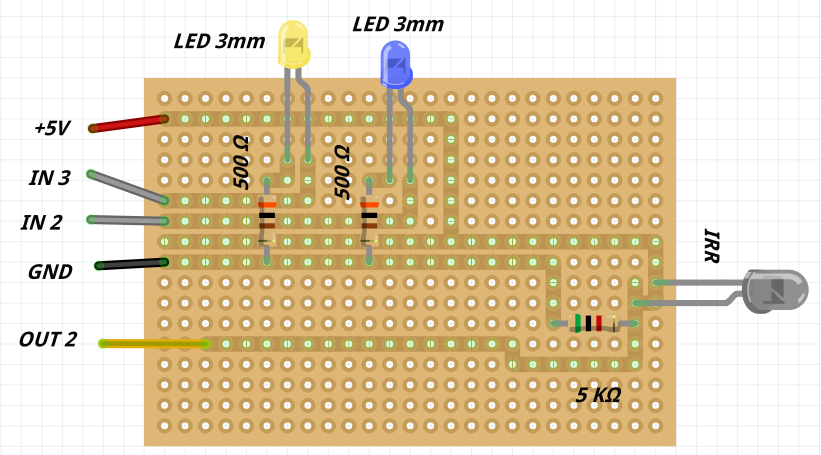
\includegraphics[width=8cm, height=5cm]{img/F5.png}  \\\\ \hline
\end{tabular}
\captionof{figure}{tarjeta perforada con el montaje del sensor de electro-recepción pasiva. Figura generada en Fritzing.}
\label{fig:Elec_Pas}
\end{Figure}
El sistema de electro-recepción pasiva como se observa en las figuras \ref{fig:Elec_Pas} y \ref{fig:Elec_Pas_placa} , consta de un diodo receptor infrarrojo o IRR, dos led de 3mm, dos resistencias de $500\Omega$, una resistencia de $5 k\Omega$, el pin IN2 es la salida al pin D10(PWM) del microcontrolador, el pin IN3 es la salida al pin D11(PWM) del microcontrolador, el pin OUT2 es la salida al pin (A0) del microcontrolador, un pin de entrada +5V y un pin de entrada a GND.

%---------------------- Placa de circuito impreso Sensor electrorecepcion pasiva
\begin{Figure}
\center
\begin{tabular}{|l|r|}
\hline
\\
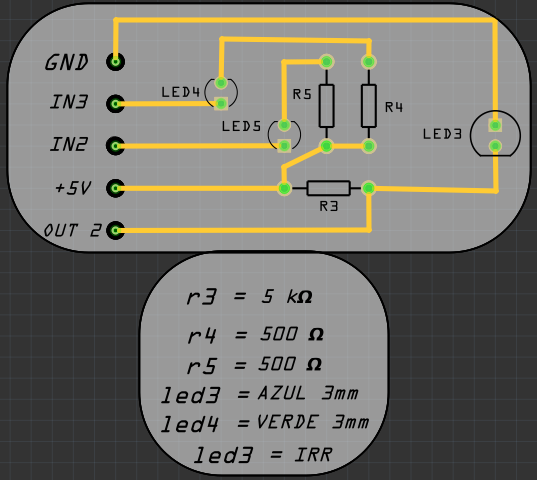
\includegraphics[width=8cm, height=5cm]{img/H2.png}  \\\\ \hline
\end{tabular}
\captionof{figure}{Placa de circuito impreso para el sensor de electro-recepción pasiva. Figura generada en Fritzing.}
\label{fig:Elec_Pas_placa}
\end{Figure}
El sensor esta calibrado para medir $40 \mu W/mV$, recolectando 4 datos por segundo, los diodos led son solo indicadores del proceso que esta realizando el microcontrolador y de la intensidad de señal recibida por el sensor, cantidad máxima medible $20 mW/\Omega$.

%--------------------------seccion electrorecpcion activa
\subsubsection{Sensor de electro-recepción activa}
El sensor de electro-recepción activa como se observa en la figura \ref{fig:recepcion-activa} . esta basado en el principio de electro-recepción activa sin barrido, el cual consiste en un sensor de recepción por reflexión, donde una fuente fotónica ubicada al lado del sensor 	envía un flujo de energía electromagnética en la longitud de onda de $940 nm$ por el espacio y al encontrar una  barrera que le impide el paso, esta interactúa con el obstáculo dando una reflexión del flujo irradiado en sentido contrario, fruto de esta interacción es la reducción de la intensidad de la señal. Ahora el sensor infrarrojo percibe esta señal transformando la energía lumínica en energía eléctrica, esta información es enviada al microcontrolador quien a su vez la envía por el bluetooth al software de control free infrarossi para su análisis. 
%------------------------Sensor electrorrecepcion activa 
\begin{Figure}
\center
\begin{tabular}{|l|r|}
\hline
\\
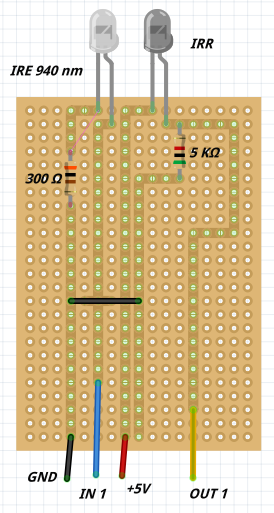
\includegraphics[width=5cm, height=7cm]{img/F4.png}  \\\\ \hline
\end{tabular}
\captionof{figure}{Esquema tarjeta perforada del radar de electro-recepción activa sin barrido, el cable de color negro es el pin de salida a tierra ( GND ), el cable de color azul es el pin de salida al pin D6(PWM) del microcontrolador,  el cable de color rojo es el pin de conexión a (+5V), el cable de color naranja es la conexión al pin $A5$ del microcontrolador. Figura generada en Fritzing.}
\label{fig:Elec_Act}
\end{Figure}
El sistema de electro-recepción activa como se observa en las figuras \ref{fig:Elec_Act} y \ref{fig:PCB_Elec_Act} , consta de un diodo receptor infrarrojo o IRR, un diodo emisor infrarrojo o IRE, una resistencia de $300\Omega$, una resistencia de $5 k\Omega$, un pin de entrada +5V y un pin de entrada a GND, el pin IN1 es la conexión al pin D6(PWM) del microcontrolador, el pin OUT1 es la salida al pin A5 del microcontrolador.
%----------------------PCB Sensor electrorecepcion activa 
\begin{Figure}
\center
\begin{tabular}{|l|r|}
\hline
\\
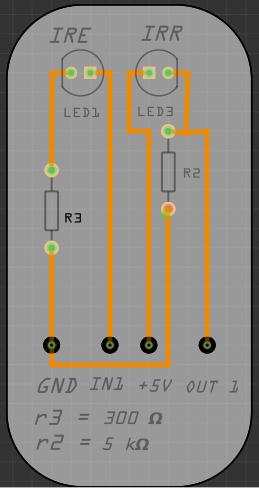
\includegraphics[width=5cm, height=7cm]{img/H1.png}  \\\\ \hline
\end{tabular}
\captionof{figure}{Placa de circuito impreso para el sensor de electro-recepción activa. Figura generada en Fritzing.}
\label{fig:PCB_Elec_Act}
\end{Figure}
El emisor infrarrojo de longitud de onda $940 nm$ tiene una densidad de flujo radiante sobre  ángulo solido de $20 mW/\Omega$.\\\\
El sensor de electro-recepción activa esta calibrado para medir $40 \mu W/mV$, recolectando 4 datos por segundo, máxima intensidad medible $20 mW/\Omega$ , con máximo alcance en la distancia de detección de 60 cm a la fuentes radiante.
%----------------------subseccion disposicion mecanica 
\subsection{Disposición mecánica}
La disposición mecánica del vehículo motorizado free infrarossi como se observa en las figuras \ref{fig:Mon_chasis_infe} ,  \ref{fig:Mon_vis_inf} , \ref{fig:Mon_meca_sup} , \ref{fig:Mon_chasis_supe} y \ref{fig:Mon_meca} , esta compuesta por un chasis de madera, dos pares de llantas, dispone de tres bases macizas forradas en velcro, para facilitar el montaje de los diferentes sensores y sistemas de control, la base del sistema de control es hueca con espacio suficiente para la bateria de $9 V$ de tipo cuadrada recargable, el montaje del vehículo,  un capó de material fommy negro para aislar el ruido en el sensor de electro-recepción activa,  dos ejes fijos, un sistema de transmisión de tipo engranaje y sistema de avance de 2 mm (únicamente  hacia adelante), los sistemas de control se puedan quitar y poner en el vehículo debido al material de velcro, el sistema de control aparte de ser móvil, puede  ser removido el microcontrolador y programado con futuras actualizaciones del firmware que provee el software free infrarossi para el vehículo motorizado infrarossi y ampliar su funcionalidad como instrumento de laboratorio, estos sensores de adquisición de datos  no solo sirven para ilustrar la propiedad de difracción, atenuación y absorción de las ondas electromagnéticas, sino que por su naturaleza activa y pasiva, podrían ser utilizados para  ilustrar la magnitud de la  aceleración gravitacional terrestre, las características en el  movimiento de un péndulo, entre otras. 
%----------------------- SECCIÓN CONTROL DE SOFTWARE 	
\section{Control de hardware a través del software free infrarossi}
%------------subsección Que es 
\subsection{¿Qué es free infrarossi?}
Free infrarossi es un  programa creado en Colombia, en la ciudad de Bogotá, como tesis de grado para optar por el titulo de licenciado en física en la Universidad Distrital Francisco José de Caldas, el cual fue desarrollado con software libre y en un entorno libre como lo es GNU-Linux, no es multiplataforma, fue diseñado únicamente para este sistema operativo; se vale de lenguajes de programación, como  C, C++, python 2.7, bash; y de programas como arduino, octave, latex, gnuplot, blueman-manager entre otros, fusionados en una interfaz amigable y fácil de utilizar. \\\\
Free infrarossi es el laboratorio virtual del instrumento de laboratorio infrarossi  que ilustra  la propiedad de difracción, atenuación y absorción de ondas electromagnéticas en el espectro infrarrojo, esta diseñado para ser utilizado tanto por  estudiantes como docentes de muy diversas ramas de las ciencias y  la ingeniería o como una herramienta muy útil para los educadores y alumnos de media vocacional.
%--------------subsección Licencia
\subsection{Licencia}
Programa de control de hardware e ilustración física de las propiedades de las ondas electromagnéticas en el espectro infrarrojo.\\\\
Copyright (C) 2016-01-01  Universidad Distrital Francisco Jose, Diego Alberto Parra Garzón, Dr. Julian Andres Salamanca Bernal. \\\\
El programa free infrarossi es software libre; puedes redistribuirlo y / o modificarlo bajo los términos de la Licencia Pública General GNU publicada por la Fundación para el Software Libre; ya sea 	la versión 3 de la Licencia, o (a su elección) cualquier versión posterior. \\\\
Este programa se distribuye con la esperanza de que sea útil, pero SIN NINGUNA GARANTÍA; ni siquiera la garantía implícita de COMERCIALIZACIÓN o IDONEIDAD PARA UN PROPÓSITO PARTICULAR. Vea la Licencia Pública General GNU para más detalles. \\\\
Debería haber recibido una copia de la Licencia Pública General de GNU junto con este programa; si no, escriba a la Free Software Foundation, Inc., 51 Franklin Street, Quinto Piso, Boston, MA 02110-1301 EE.UU..\\\\
Si usted hace alguna modificación en esta aplicación, deberá siempre mencionar el autor original de la misma.
%------------.subsección instalación 
\subsection{Instalación}
La instalación de este software es el mismo para distribuciones basadas en Debian\footnote{Pagina oficial proyecto Debian https://www.debian.org/}.
\begin{enumerate}
\item[a.] Abrir una terminal\footnote{Procedimiento: http://www.comoinstalarlinux.com/como-abrir-una-terminal-en-ubuntu-linux-mint-centos-debian/} como se observa en la figura \ref{fig:Comandos_terminal} y escribir sin comillas $"$sudo su$"$ y luego oprimir la tecla enter.\\
\item[b.] Escribir la contraseña de administrador, presione enter.\\
\item[c.] Escribir sin comillas $"$aptitude install -y git$"$, presione enter.\\
\item[d.] Escribir sin comillas $"$cd Documentos$"$ presione enter.\\
\item[e.] Escribir sin comillas $"$git  clone  https://github.com/\\Nombre$\_$Usuario/Free-infrarossi$"$, oprimir enter.\\
\item[f.] Escribir sin comillas $”$chmod +777 Free-infrarossi$”$, presione la tecla enter.\\
\item[g.] Cerrar la terminal y dirigirse al navegador de archivos en la carpeta Documentos/Free-infrarossi/install, como se observa en la figura \ref{fig:Navegador_archivos} .\\
\item[h.] Dar click derecho del mouse en el archivo instalador.py como se observa en las figuras \ref{fig:propiedades1} y \ref{fig:propiedades2} , click izquierdo en la opción propiedades; en la pestaña de general debe decir abrir archivo con python 2.7 y en la pestaña permisos debe estar seleccionada la casilla permitir ejecutar este archivo como programa, de no ser cambiar las opciones.
\item[i.] Cerrar la ventana y abrir el archivo INSTALADOR.py.
\item[j.] Escribir la clave administrador y presionar enter.
\item[k.] Escribir  1 y presionar enter.
\item[l.] Escribir nuevamente 1 y enter.
\item[m.] Una vez finalizada la instalación hay que reiniciar el pc.
\end{enumerate}
%--------------------comandos en terminal

\begin{Figure}	
\center
\begin{tabular}{|l|r|}
\hline
\\
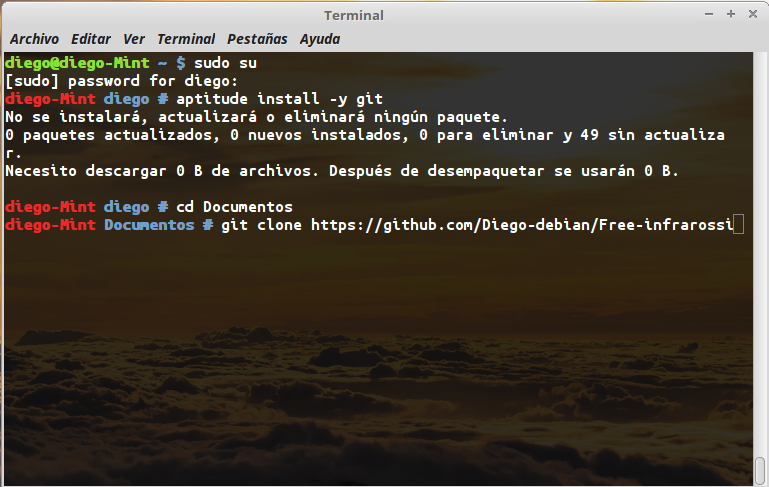
\includegraphics[width=8cm, height=6cm]{img/S_install2.png} \\\\ \hline
%10. \\ \hline 
\end{tabular}
\captionof{figure}{Instalación, comandos en terminal de Linux mint 17.2}
\label{fig:Comandos_terminal}
\end{Figure}
%--------------------carpeta install
\begin{Figure}	
\center
\begin{tabular}{|l|r|}
\hline
\\
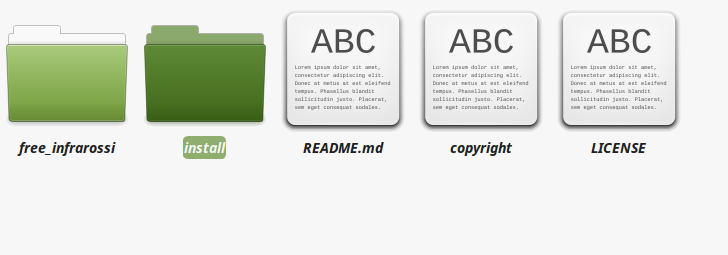
\includegraphics[width=8cm, height=3cm]{img/S_install.png} \\\\ \hline
%10. \\ \hline 
\end{tabular}
\captionof{figure}{Instalación, vista navegador de archivos.}
\label{fig:Navegador_archivos}
\end{Figure}
%--------------------propiedades1
\begin{Figure}	
\center
\begin{tabular}{|l|r|}
\hline
\\
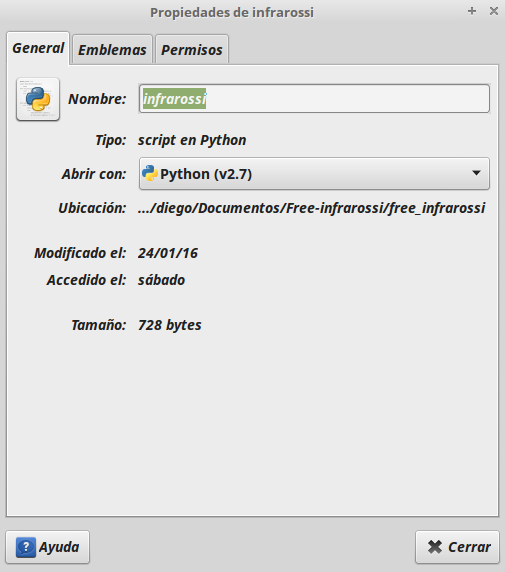
\includegraphics[width=8cm, height=6cm]{img/S_propiedades1.png} \\\\ \hline
%10. \\ \hline 
\end{tabular}
\captionof{figure}{Instalación, propiedades free infrarossi}
\label{fig:propiedades1}
\end{Figure}
%--------------------propiedades 2
\begin{Figure}	
\center
\begin{tabular}{|l|r|}
\hline
\\
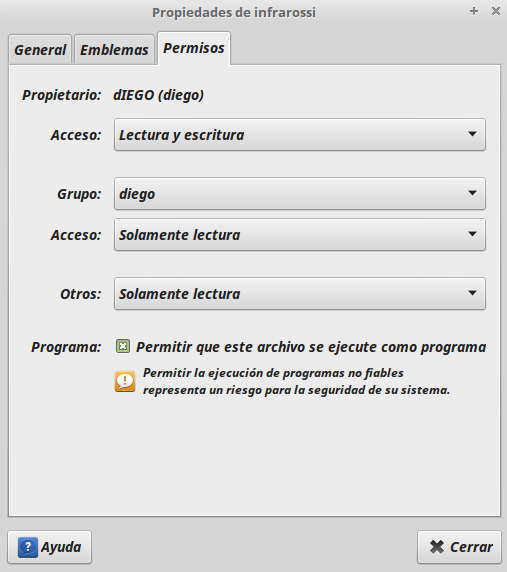
\includegraphics[width=8cm, height=6cm]{img/S_propiedades2.png} \\\\ \hline
%10. \\ \hline 
\end{tabular}
\captionof{figure}{Instalación, propiedades free infrarossi}
\label{fig:propiedades2}
\end{Figure}
%_------------------------------subsección Primer uso
\subsection{Primer uso free infrarossi}
Abrir una terminal del S.O. escribir en la terminal sin comillas $'infrarossi'$ , oprimir la tecla enter, escribir la clave de administrador y se despliega la ventana del software free infrarossi, como se aprecia en la figura \ref{fig:Firmware_1}.
\begin{Figure}	
\center
\begin{tabular}{|l|r|}
\hline
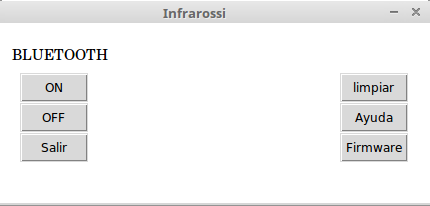
\includegraphics[width=8cm, height=4cm]{img/infrarossi.png} \\ \hline
%10. \\ \hline 
\end{tabular}
\captionof{figure}{Instalación, comandos en terminal de Linux mint 17.2}
\label{fig:Firmware_1}
\end{Figure}
\subsection{Carga de firmware en integrado atmega 328}
La ventana del programa free infrarossi, en la parte inferior derecha hay tres botones, oprimir el botón de firmware  como se muestra en la figura \ref{fig:carga_firmware} , y conectar la tarjeta micro controladora arduino uno al pc; oprimir el botón continuar y esperar que cargue el firmware en la tarjeta, una vez hecho esto retirar el micro controlador de la tarjeta y colocarlo en el montaje del vehículo.
\begin{Figure}	
\center
\begin{tabular}{|l|r|}
\hline
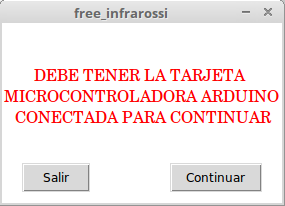
\includegraphics[width=8cm, height=4cm]{img/firmware.png} \\ \hline
\end{tabular}
\captionof{figure}{Ventana de instalación del firmware, que ofrece el software free infrarossi, para el vehículo motorizado infrarossi.}
\label{fig:carga_firmware}
\end{Figure}
\subsection{Test del instrumento infrarossi y su software de control free infrarossi}
\ref{infrarossi}



\begin{thebibliography}{99}
\bibitem{ELECTRORRECPCION} Pedraja, F. (2012). Modelo computacional de Gymnotus omarorum: Un pez eléctrico de pulso con órgano distribuido.
\bibitem{ARDUINO} Atmel. (2015). Atmel 8-BIT Microcontroller with 4/8/16/32KBYTES in-system programmable flash. atmega328P-PU data sheet [On line]. Disponible en: \\ http://www.atmel.com/Images/Atmel-8271-8-bit-AVR\\-Microcontroller-ATmega48A-48PA-88A-88PA-168A-16\\8PA-328-328P\_datasheet\_Summary.pdf
\bibitem{REGULADOR} Semiconductor, F. (2012). LM7805 Data Sheet. [Online]. Disponible en:\\ http://pdf.datasheetcatalog.net/datasheet/fairchild/L\\M7805.pdf
\bibitem{TIP122} Semiconductor, F. (2008). Tip120/tip121/tip122 npn epitaxial darlington transistor. TIP120 datasheet, Oct. [On line]. Disponible en:\\ http://pdf.datasheetcatalog.net/datasheet/fairchild/\\TIP122.pdf.
\bibitem{PHOTOTRANSISTOR} Phototransistor T1. (2006). Pt333-3B Data Sheet. [Online]. Disponible en:\\ http://media.digikey.com/pdf/Data\%20Sheets/Everli\\ght\%20PDFs/PT333-3B.pdf
% \bibitem{DIODO}  Hoja de datos diodo regulador 1N4001. http://pdf.datasheetcatalog.net/datasheet/lrc/\\1N4001.pdf
%\bibitem{INFRARED} Hoja de datos del diodo, emisor. \\ http://www.datasheetarchive.com/dlmain/Datasheets\\-31/DSA-617614.pdf
\bibitem{FRITZING} Knörig, A., Wettach, R., \& Cohen, J. (2009, February). Fritzing: a tool for advancing electronic prototyping for designers. In Proceedings of the 3rd International Conference on Tangible and Embedded Interaction. ACM.
\bibitem{PYTHON} Gift, N., \& Jones, J. M. (2008). Python for Unix and Linux system administration. ``O'Reilly Media, Inc.".
\bibitem{CIRCUITOS} Alexander, C. K., Sadiku, M. N., Bermúdez, A. V., \& Pedraza, C. R. C. (2006). Fundamentos de circuitos eléctricos. McGraw-Hill. 
\end{thebibliography}
\end{multicols}
%----------------------------------------------------------ANEXOS
%\clearpage % o \cleardoublepage
\selectlanguage{spanish}
\appendix
\addappheadtotoc
\appendixpage
%--------------------seccion montaje electrico
\section{Diseño eléctrico}
%--------------Montaje electrico, esquema equivalente
\subsection{Esquema eléctrico equivalente del vehículo}
\begin{Figure}	
\center
\fbox{
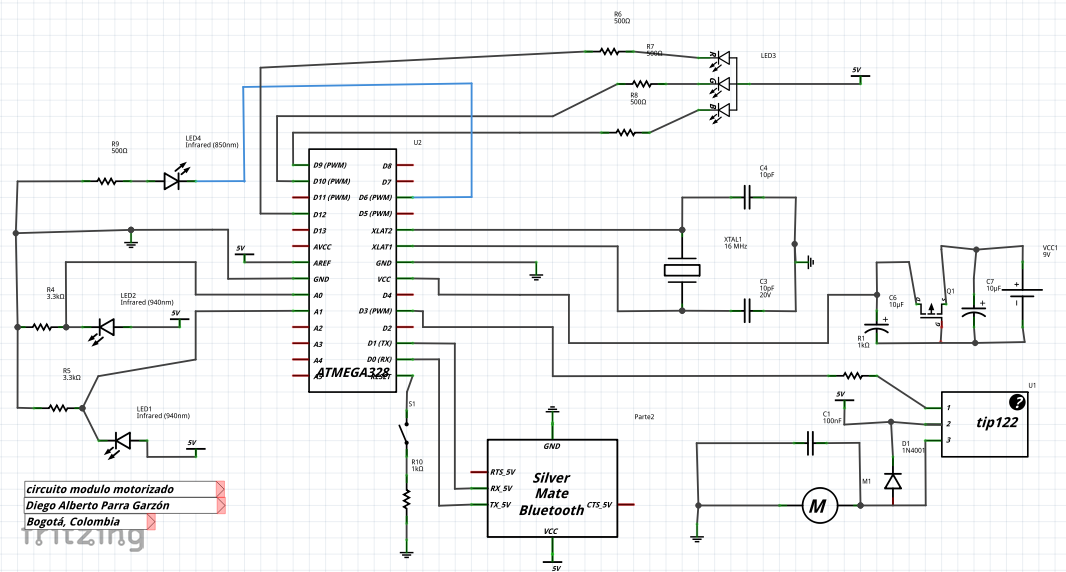
\includegraphics[width=17cm, height=13cm, angle=90]{img/esquemap.png} 
	}
\captionof{figure}{Esquema eléctrico equivalente del vehículo.}
\label{fig:cir_elec}
\end{Figure}
%--------------Montaje electrico, montaje en protoboard 
\subsection{Montaje eléctrico en protoboard}
\begin{Figure}	
\center
\fbox{
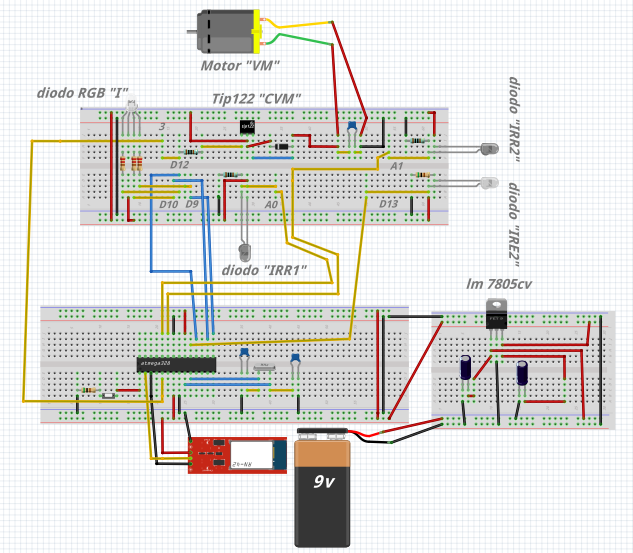
\includegraphics[width=17cm, height=13cm, angle=90]{img/montajep.png} 
	}
\captionof{figure}{Montaje en protoboard.}
\label{fig:cir_proto_elec}
\end{Figure}
%--------------Montaje electrico, sistema control de hardware
\subsection{Montaje eléctrico, sistema control de hardware}
\begin{Figure}	
\center
\fbox{
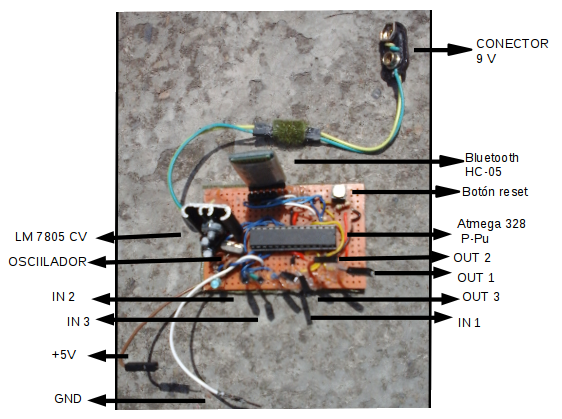
\includegraphics[width=17cm, height=13cm, angle=0]{img/TF1.png} 
	}
\captionof{figure}{Sistema control de hardware, con modulador de señal LM 7805cv, modulador de frecuencia con oscilador 12 Mhz, el pin IN2 es la conexión a led de color 3mm,  el pin IN3 es la conexión a led de color 3mm, pin de salida a +5v, pin de salida a GND, modulo bluetooth hc-05, botón de reinicio, microcontrolador atmega 328P-PU, el pin OUT1 es la salida al sensor de electro-recepción activa, el pin OUT2 es la salida al sensor de electro-recepción pasiva, el pin OUT3 es el pin de salida al sistema de control de velocidad, el pin IN1 es la salida al diodo emisor infrarrojo.}
\label{fig:control_hardware}
\end{Figure}
%--------------Montaje eléctrico, sistema control avance del vehiculo
\subsection{Montaje eléctrico, sistema control de avance del vehículo infrarossi}
\begin{Figure}	
\center
\fbox{
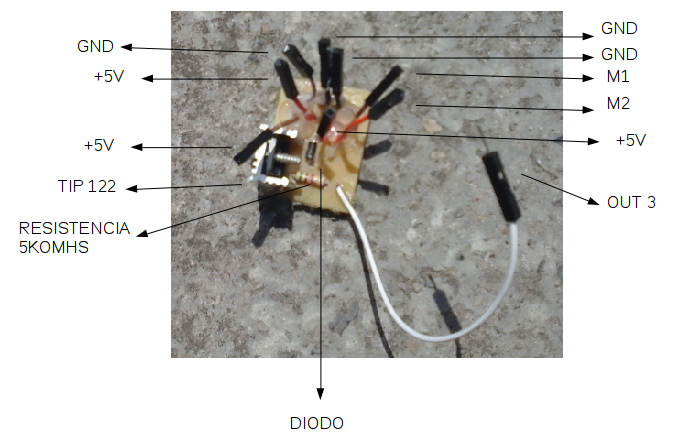
\includegraphics[width=17cm, height=13cm, angle=0]{img/TF2.png} 
	}
\captionof{figure}{Sistema control de avance del vehículo infrarossi, consta de dos salidas a GND, dos salidas a +5V, una entrada a GND, una entrada a +5V, un tip 122, una resistencia de $5k\Omega$, diodo 1N4001, el pin OUT3 es la salida al pin D3(PWM) del microcontrolador atmega, salida M1 para el motor, salida M2 para el motor.}
\label{fig:control_avance}
\end{Figure}
%--------------Montaje eléctrico, sensor electro-recepción pasiva 
\subsection{Montaje eléctrico, sensor electro-recepción pasiva}
\begin{Figure}	
\center
\fbox{
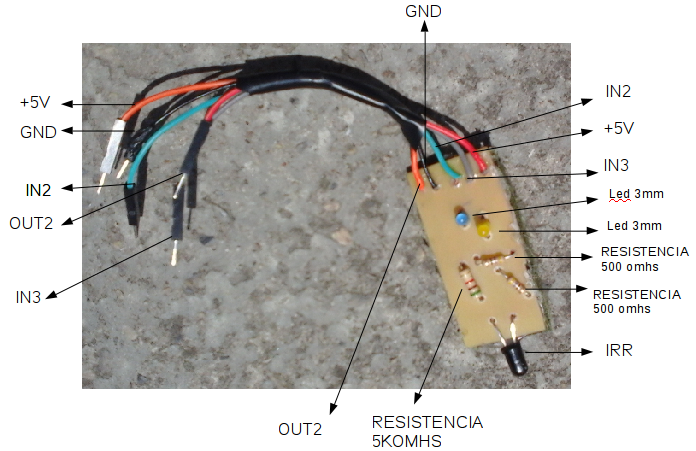
\includegraphics[width=17cm, height=13cm, angle=0]{img/TF3.png} 
	}
\captionof{figure}{El sistema de electro-recepción pasiva consta de un diodo receptor infrarrojo o IRR, dos led de 3mm, dos resistencias de $500\Omega$, una resistencia de $5 k\Omega$, el pin IN2 es la salida al pin D10(PWM) del microcontrolador, el pin IN3 es la salida al pin D11(PWM) del microcontrolador, el pin OUT2 es la salida al pin (A0) del microcontrolador, un pin de entrada +5V y un pin de entrada a GND.}
\label{fig:recepcion-pasiva}
\end{Figure}
%--------------Montaje eléctrico, sensor electro-recepción activa 
\subsection{Montaje eléctrico, sensor electro-recepción activa}
\begin{Figure}	
\center
\fbox{
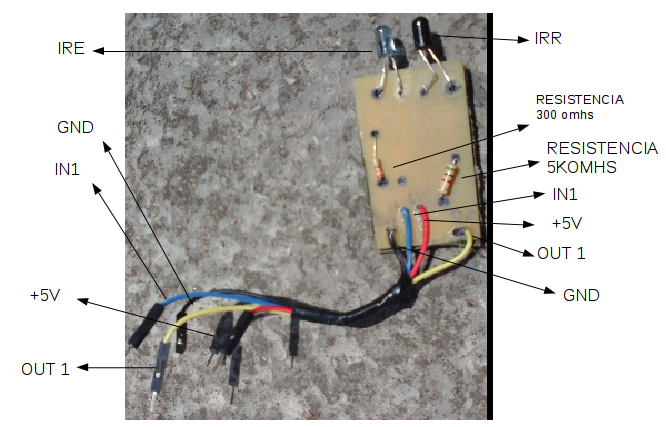
\includegraphics[width=17cm, height=13cm, angle=0]{img/TF4.png} 
	}
\captionof{figure}{El sistema de electro-recepción activa consta de un diodo receptor infrarrojo o IRR, un diodo emisor infrarrojo o IRE, una resistencia de $300\Omega$, una resistencia de $5 k\Omega$, un pin de entrada +5V y un pin de entrada a GND, el pin IN1 es la conexión al pin D6(PWM) del microcontrolador, el pin OUT1 es la salida al pin A5 del microcontrolador.}
\label{fig:recepcion-activa}
\end{Figure}
%--------------------seccion montaje mecanico
\section{Diseño mecánico}
%--------------Montaje mecánico, dimensiones del chasis.
\subsection{Montaje mecánico, dimensiones del chasis.}
\begin{Figure}	
\center
\fbox{
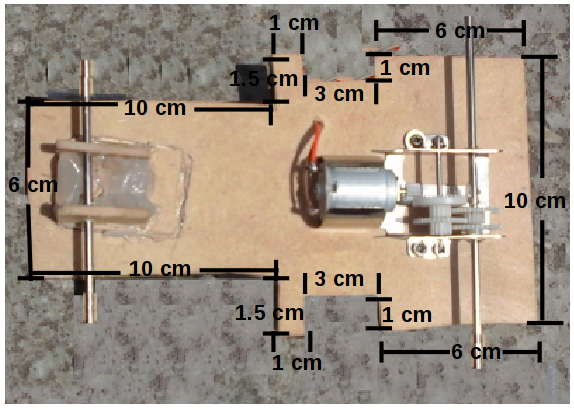
\includegraphics[width=17cm, height=13cm, angle=0]{img/TF7.png} 
	}
\captionof{figure}{Chasis  de madera con dimensiones en centímetros, la caja del eje delantero tiene dimensiones dos centímetros de ancho, 3 centímetros de largo y 2,5 centímetros de alto; el eje delantero debe estar a  1 centímetro de separación del chasis.}
\label{fig:Mon_chasis_infe}
\end{Figure}
%-------------------Montaje mecánico, vista inferior
\subsection{Montaje mecánico, vista inferior}
\begin{Figure}	
\center
\fbox{
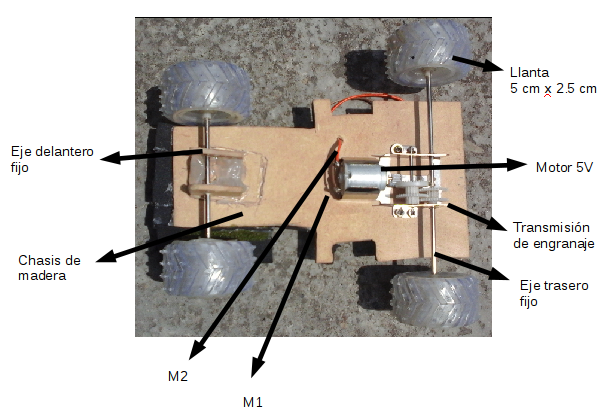
\includegraphics[width=18cm, height=13cm, angle=0]{img/TF6.png} 
	}
\captionof{figure}{Vista inferior del vehículo con eje delantero fijo, eje trasero fijo, transmisión de engranaje, motor de 5 V,  llantas de 5 cm de diámetro por   2.5 de ancho, conexión del motor M1 y conexión del motor M2.}
\label{fig:Mon_vis_inf}
\end{Figure}
%--------------Montaje mecánico, vista superior.
\subsection{Montaje mecánico, vista superior}
\begin{Figure}	
\center
\fbox{
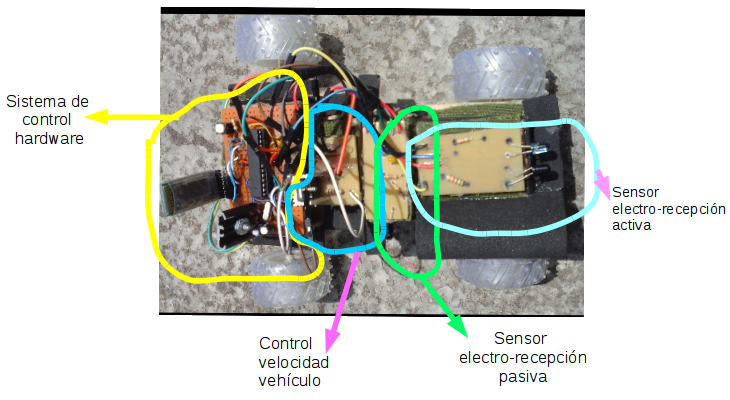
\includegraphics[width=18cm, height=12cm, angle=0]{img/TF5.png} 
	}
\captionof{figure}{Vista superior del vehículo donde se observa el sistema de control de hardware, el sistema de control de avance del vehículo, el sensor de electro-recepción pasiva y el sensor de electro-recepción activa.}
\label{fig:Mon_meca_sup}
\end{Figure}
%--------------Montaje mecánico, vista superior del chasis.
\subsection{Montaje mecánico, vista superior del chasis.}
\begin{Figure}	
\center
\fbox{
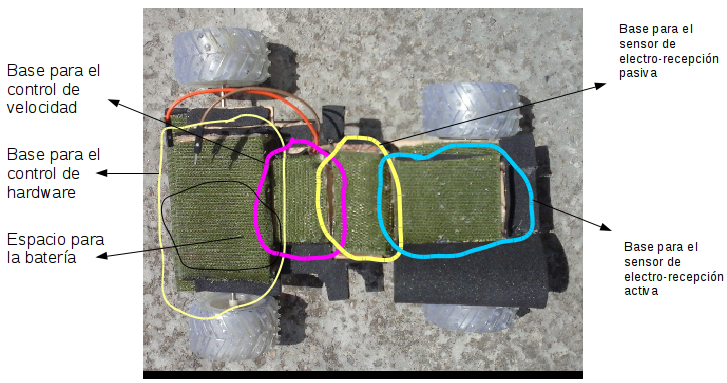
\includegraphics[width=18cm, height=12cm, angle=0]{img/TF8.png} 
	}
\captionof{figure}{Chasis vista superior las bases tienen las mismas dimensiones de los sensores tanto de ancho como de largo, el alto de las bases de 1.5 centímetros, con velcro, la base para el control de hardware tiene 2.3 cm de alto pues debajo de esta hay un espacio para guardar la batería de 9 voltios.}
\label{fig:Mon_chasis_supe}
\end{Figure}
%--------------Montaje mecánico.
\subsection{Montaje mecánico.}
\begin{Figure}	
\center
\fbox{
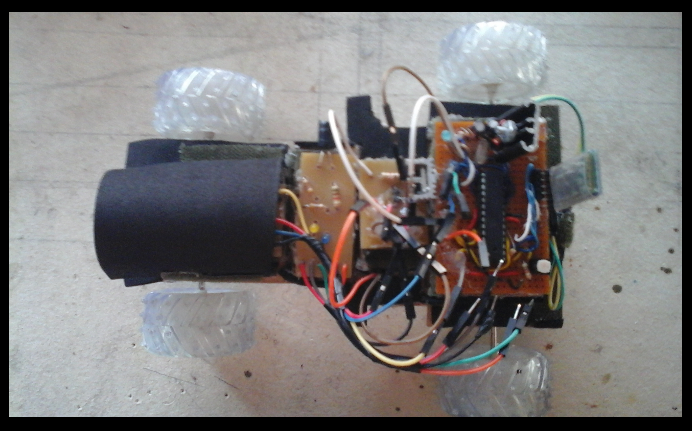
\includegraphics[width=18cm, height=12cm, angle=0]{img/F9.png} 
	}
\captionof{figure}{Chasis vista superior las bases tienen las mismas dimensiones de los sensores tanto de ancho como de largo, el alto de las bases es de 1.5 centímetros, con velcro, la base para el control de hardware tiene 2.3 cm de alto pues debajo de esta hay un espacio para guardar la batería de 9 voltios.}
\label{fig:Mon_meca}
\end{Figure}
%----------------seccion software
\newpage
\section{Códigos del programa free infrarrosi}
%------------------------LICENSE
\subsection{LICENSE}
Este código comienza en la pagina que sigue.
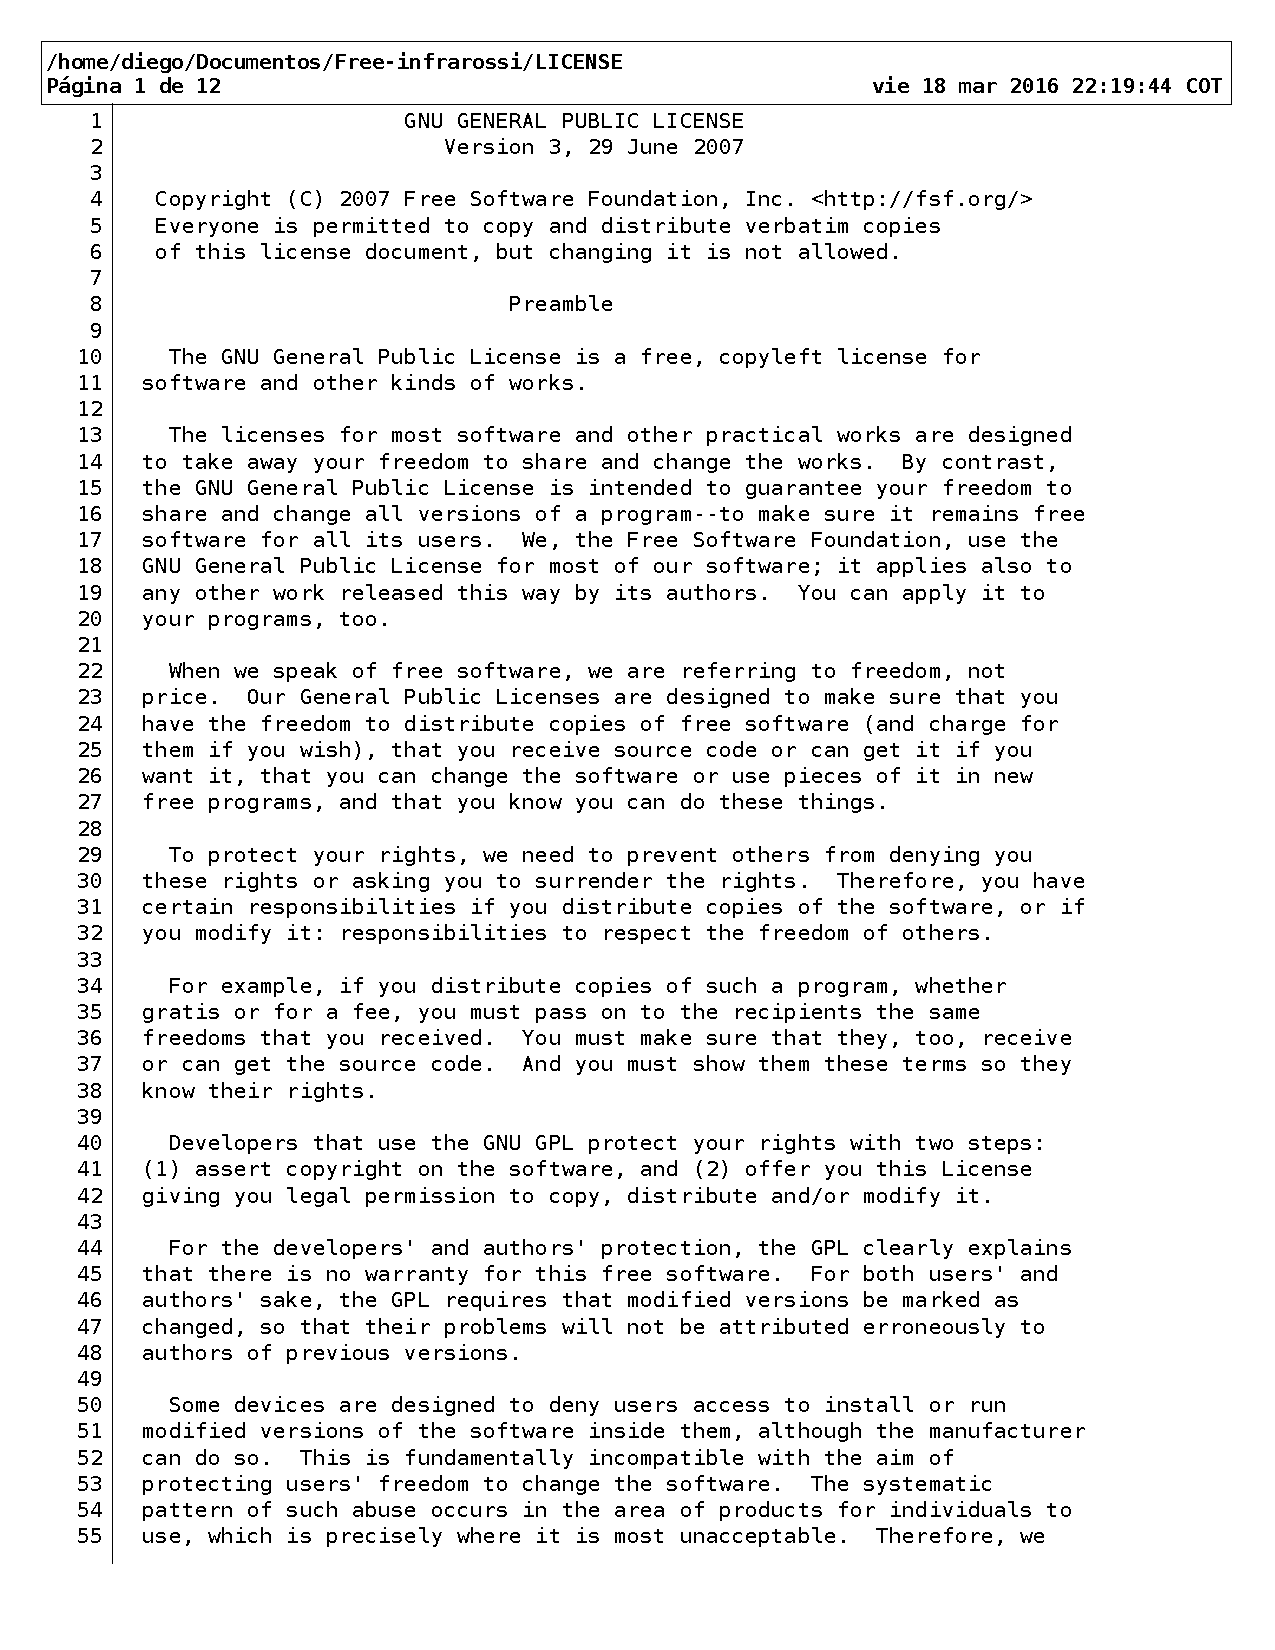
\includepdf[pages=-,scale=1,pagecommand={}]{LICENSE.pdf} 
%------------------------copyright
\subsection{copyright}
Este código comienza en la pagina que sigue.
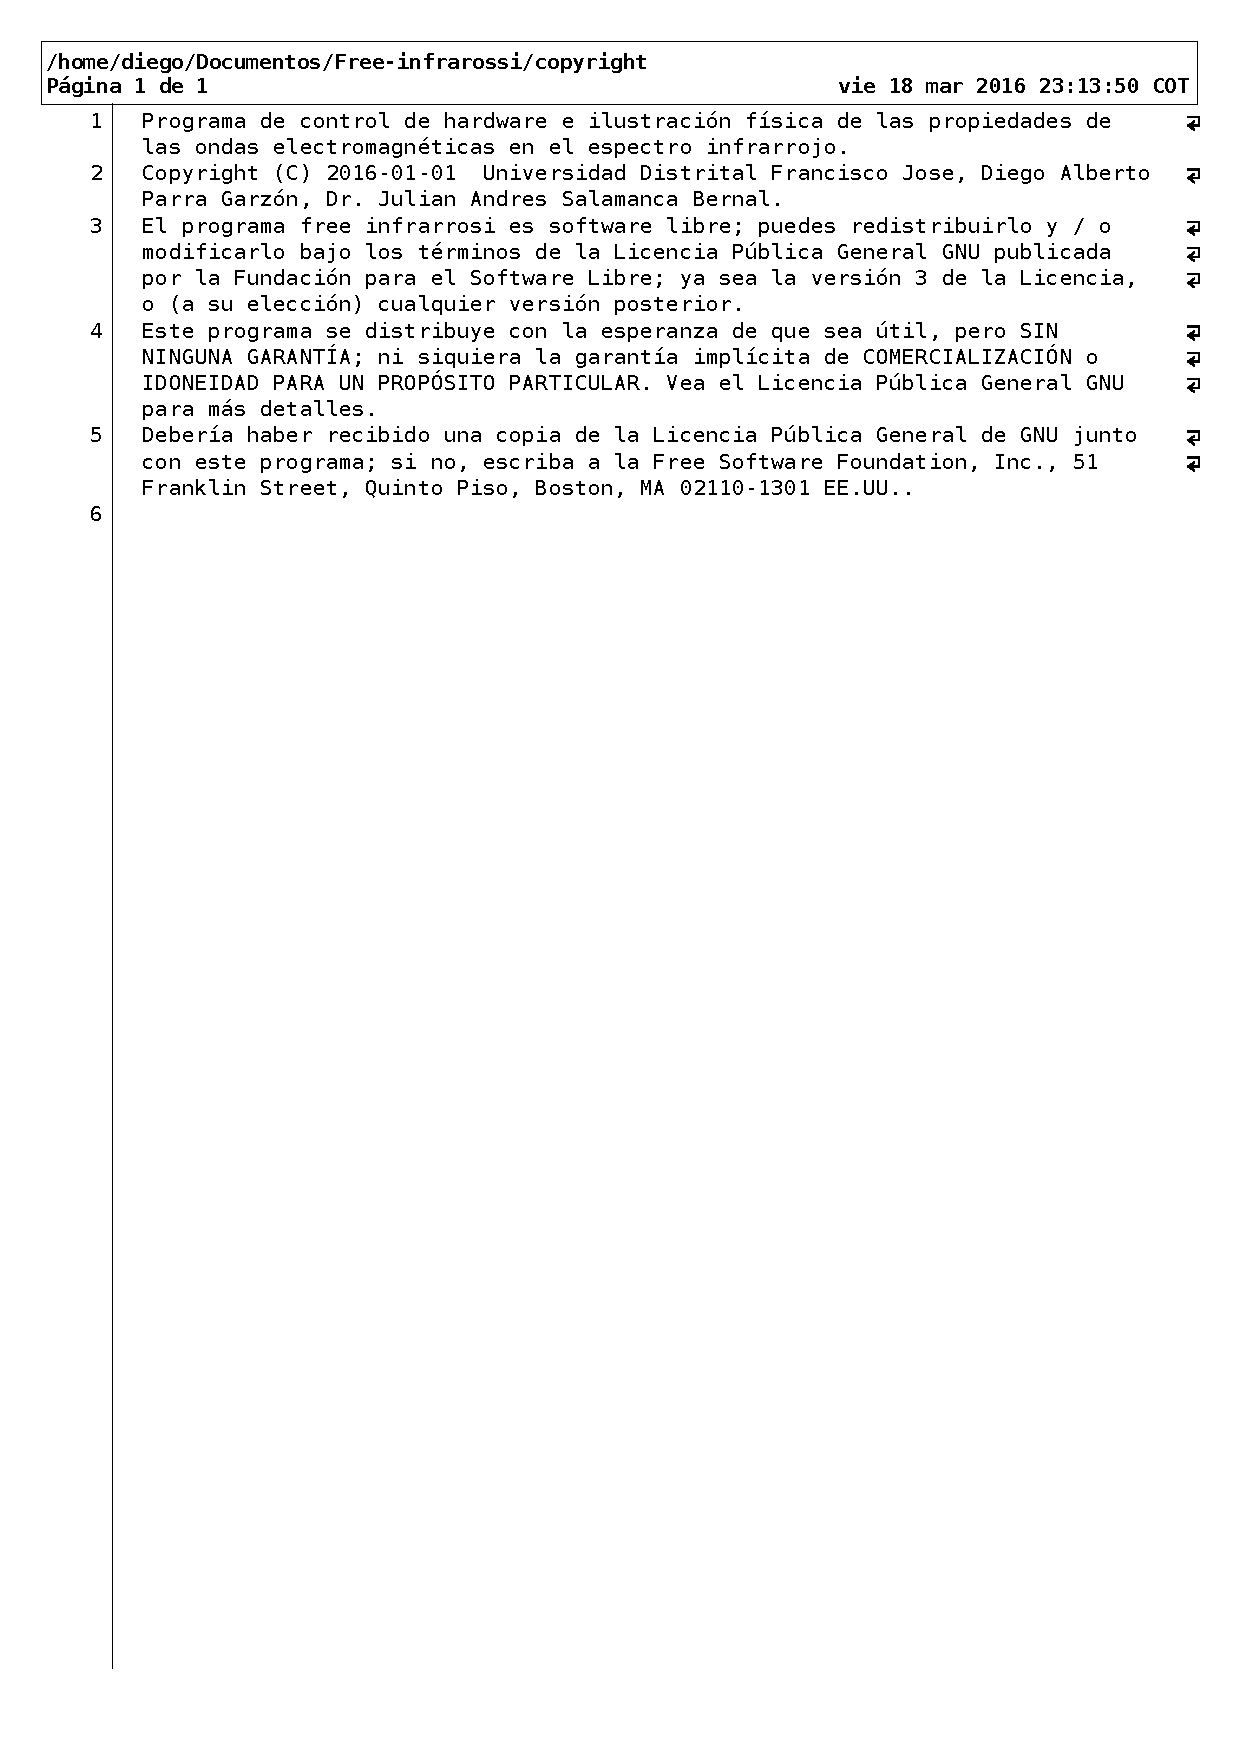
\includepdf[pages=-,scale=1,pagecommand={}]{copyright.pdf} 
%------------------------README.md
\subsection{README.md}
Este código comienza en la pagina que sigue.
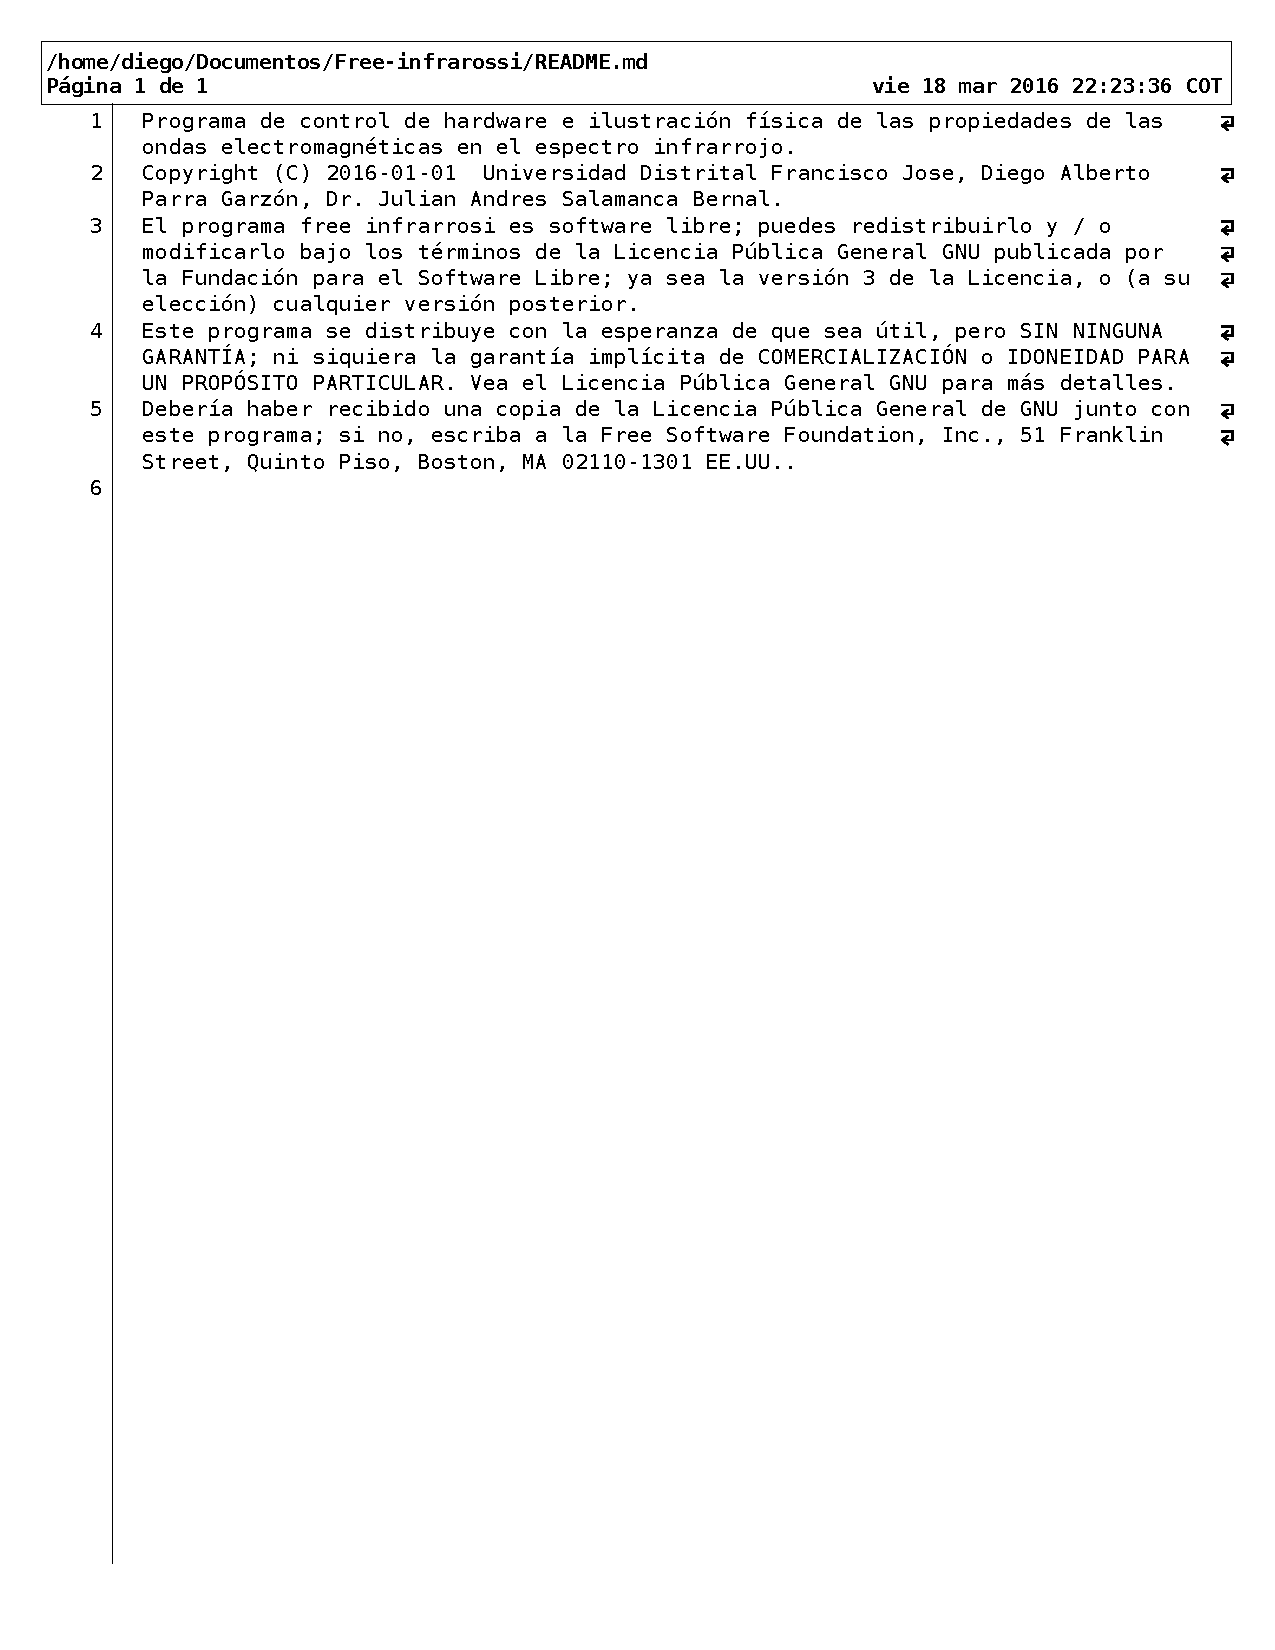
\includepdf[pages=-,scale=1,pagecommand={}]{README.pdf} 
%------------------------instalador.py
\subsection{instalador.py}
Este código comienza en la pagina que sigue.
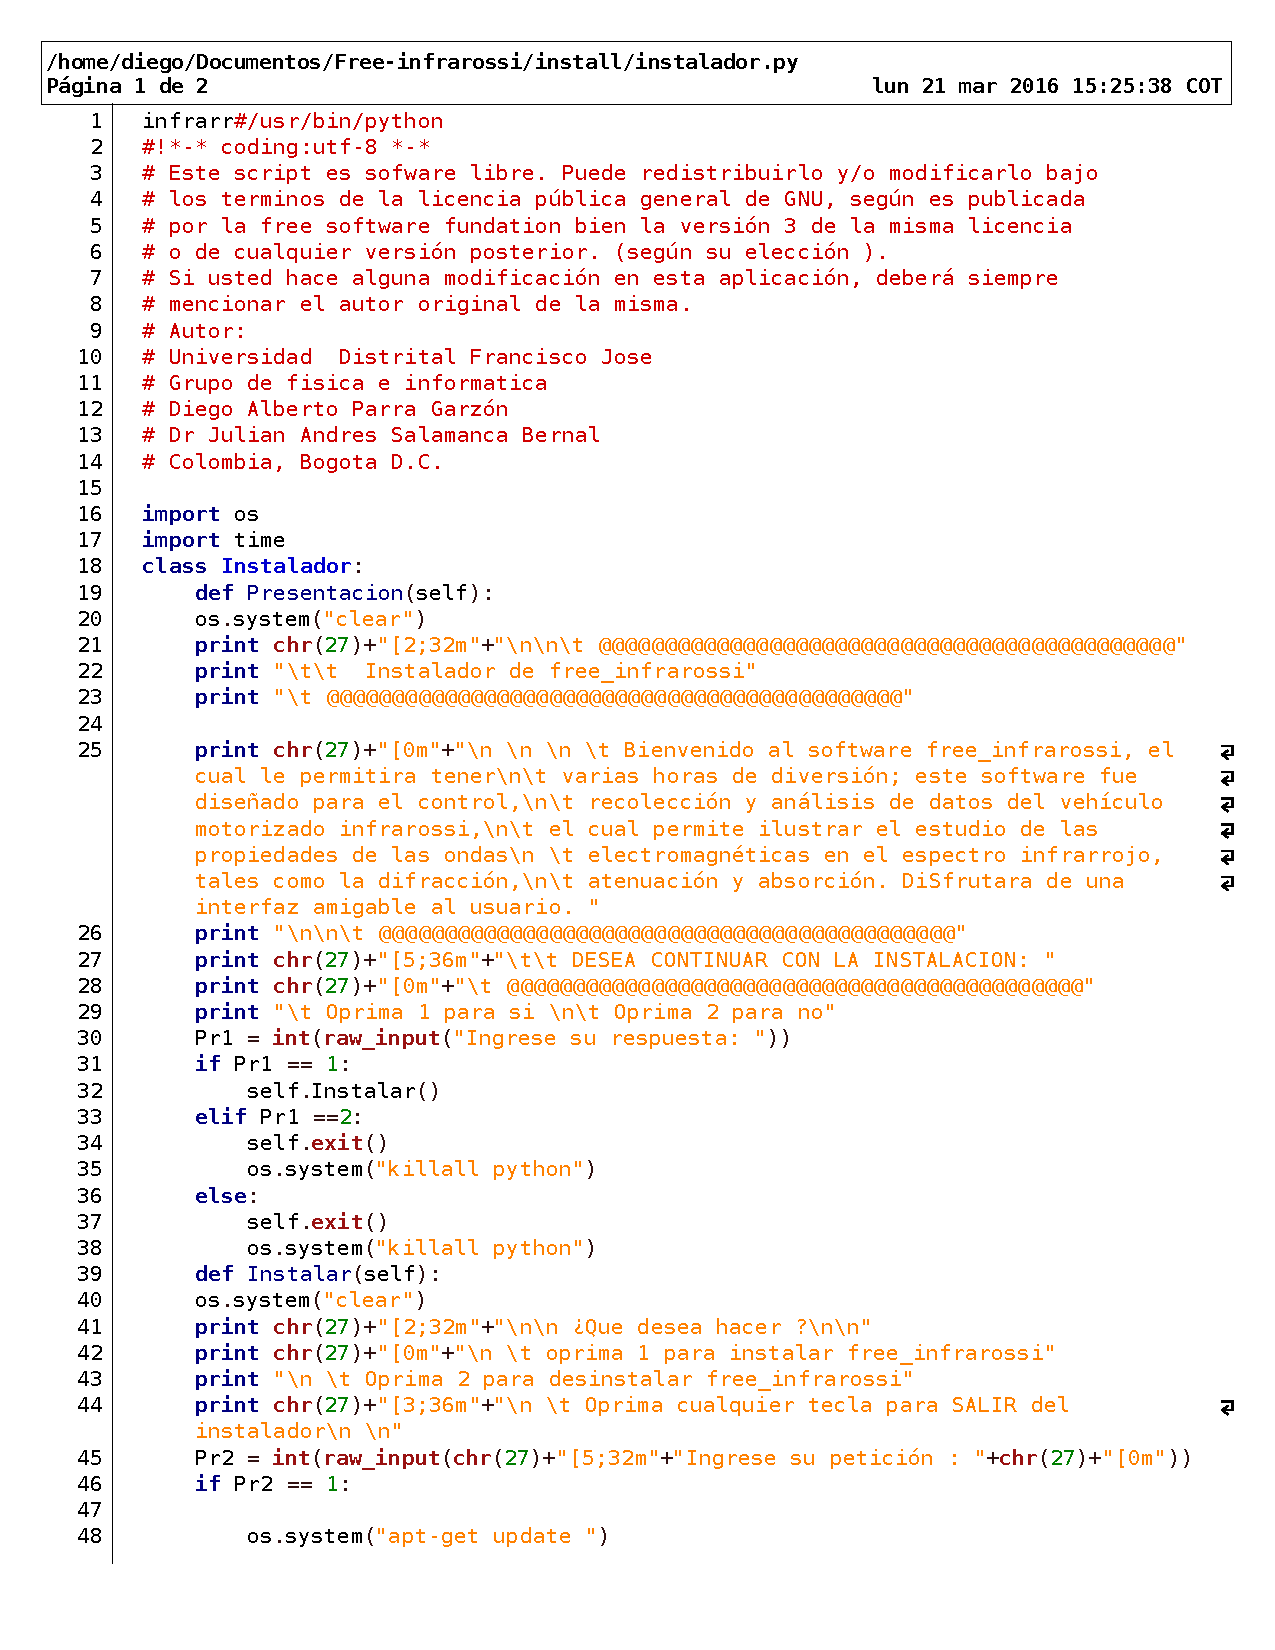
\includepdf[pages=-,scale=1,pagecommand={}]{instaladorpy.pdf} 
%------------------------INSTALADOR.py
\subsection{INSTALADOR.py}
Este código comienza en la pagina que sigue.
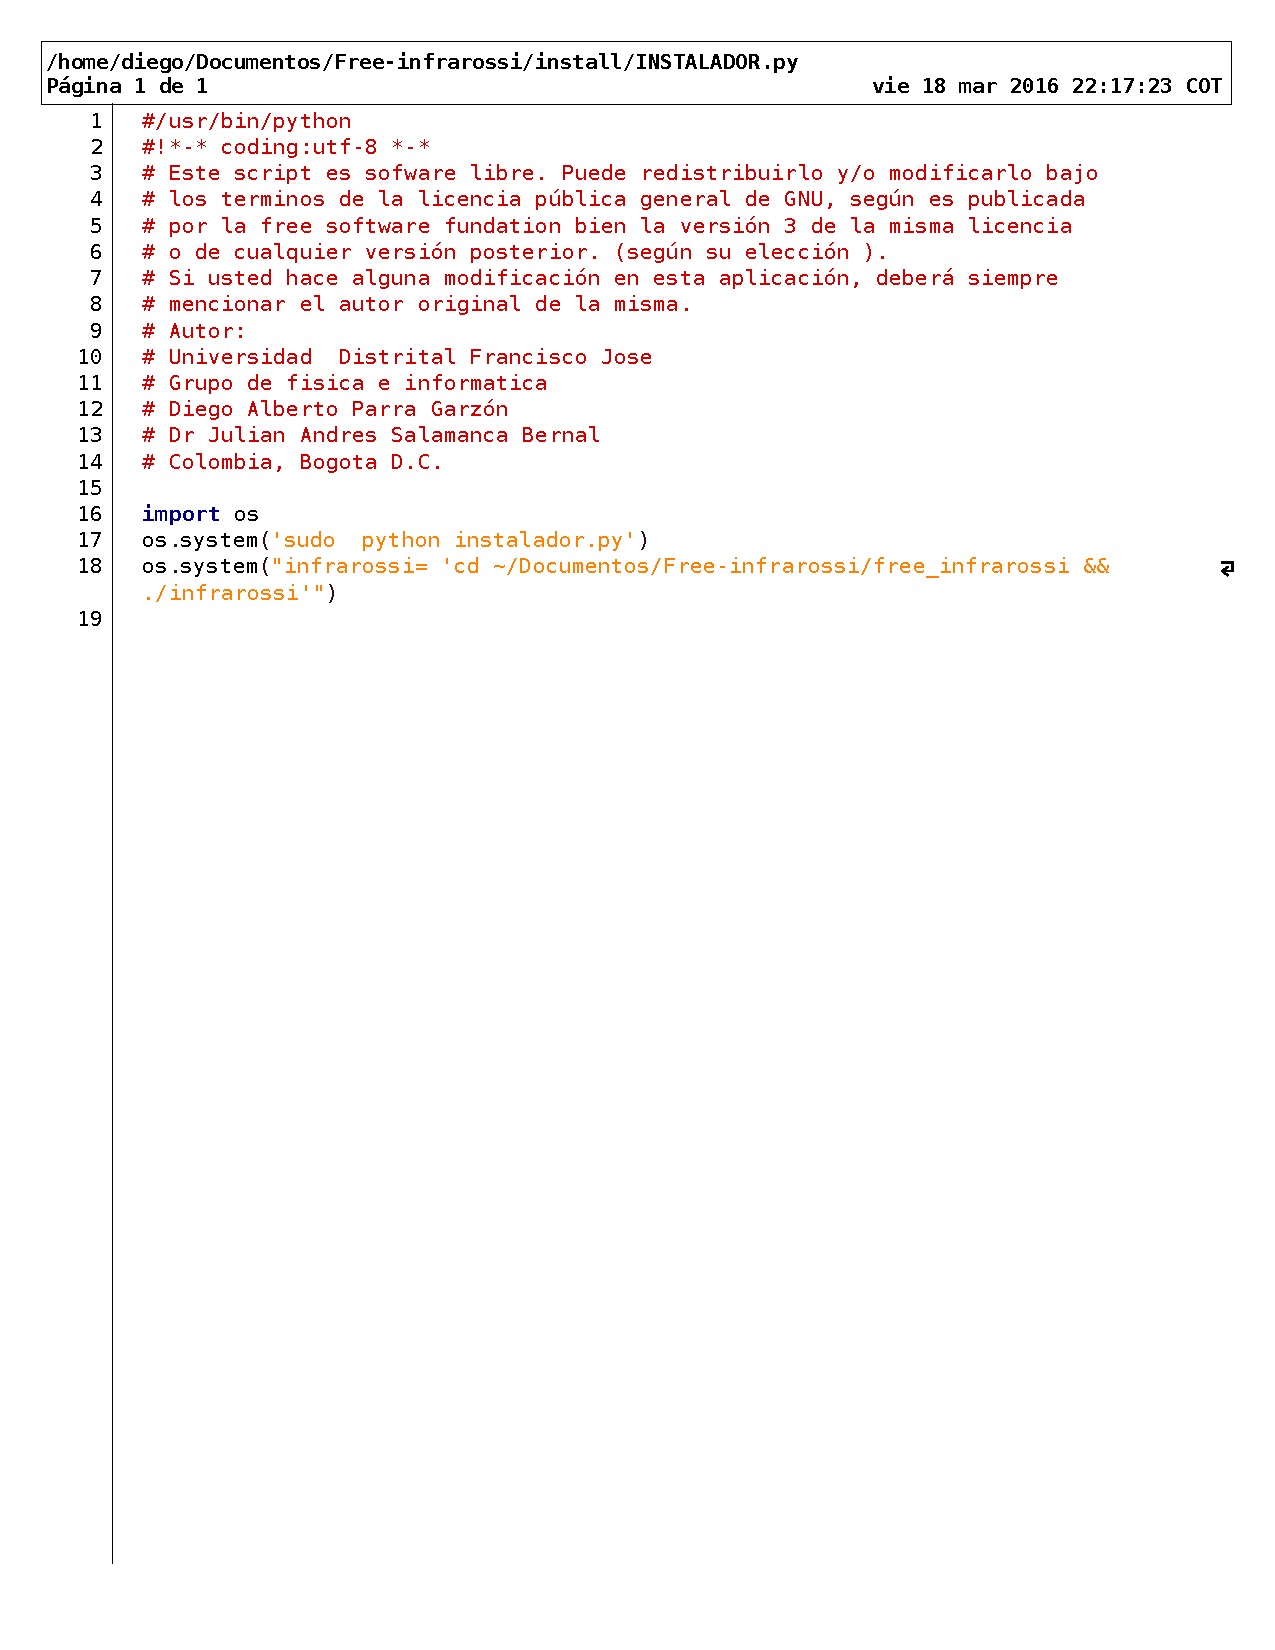
\includepdf[pages=-,scale=1,pagecommand={}]{INSTALADOR.pdf}
%------------------------unistall.py
\subsection{unistall.py}
Este código comienza en la pagina que sigue.
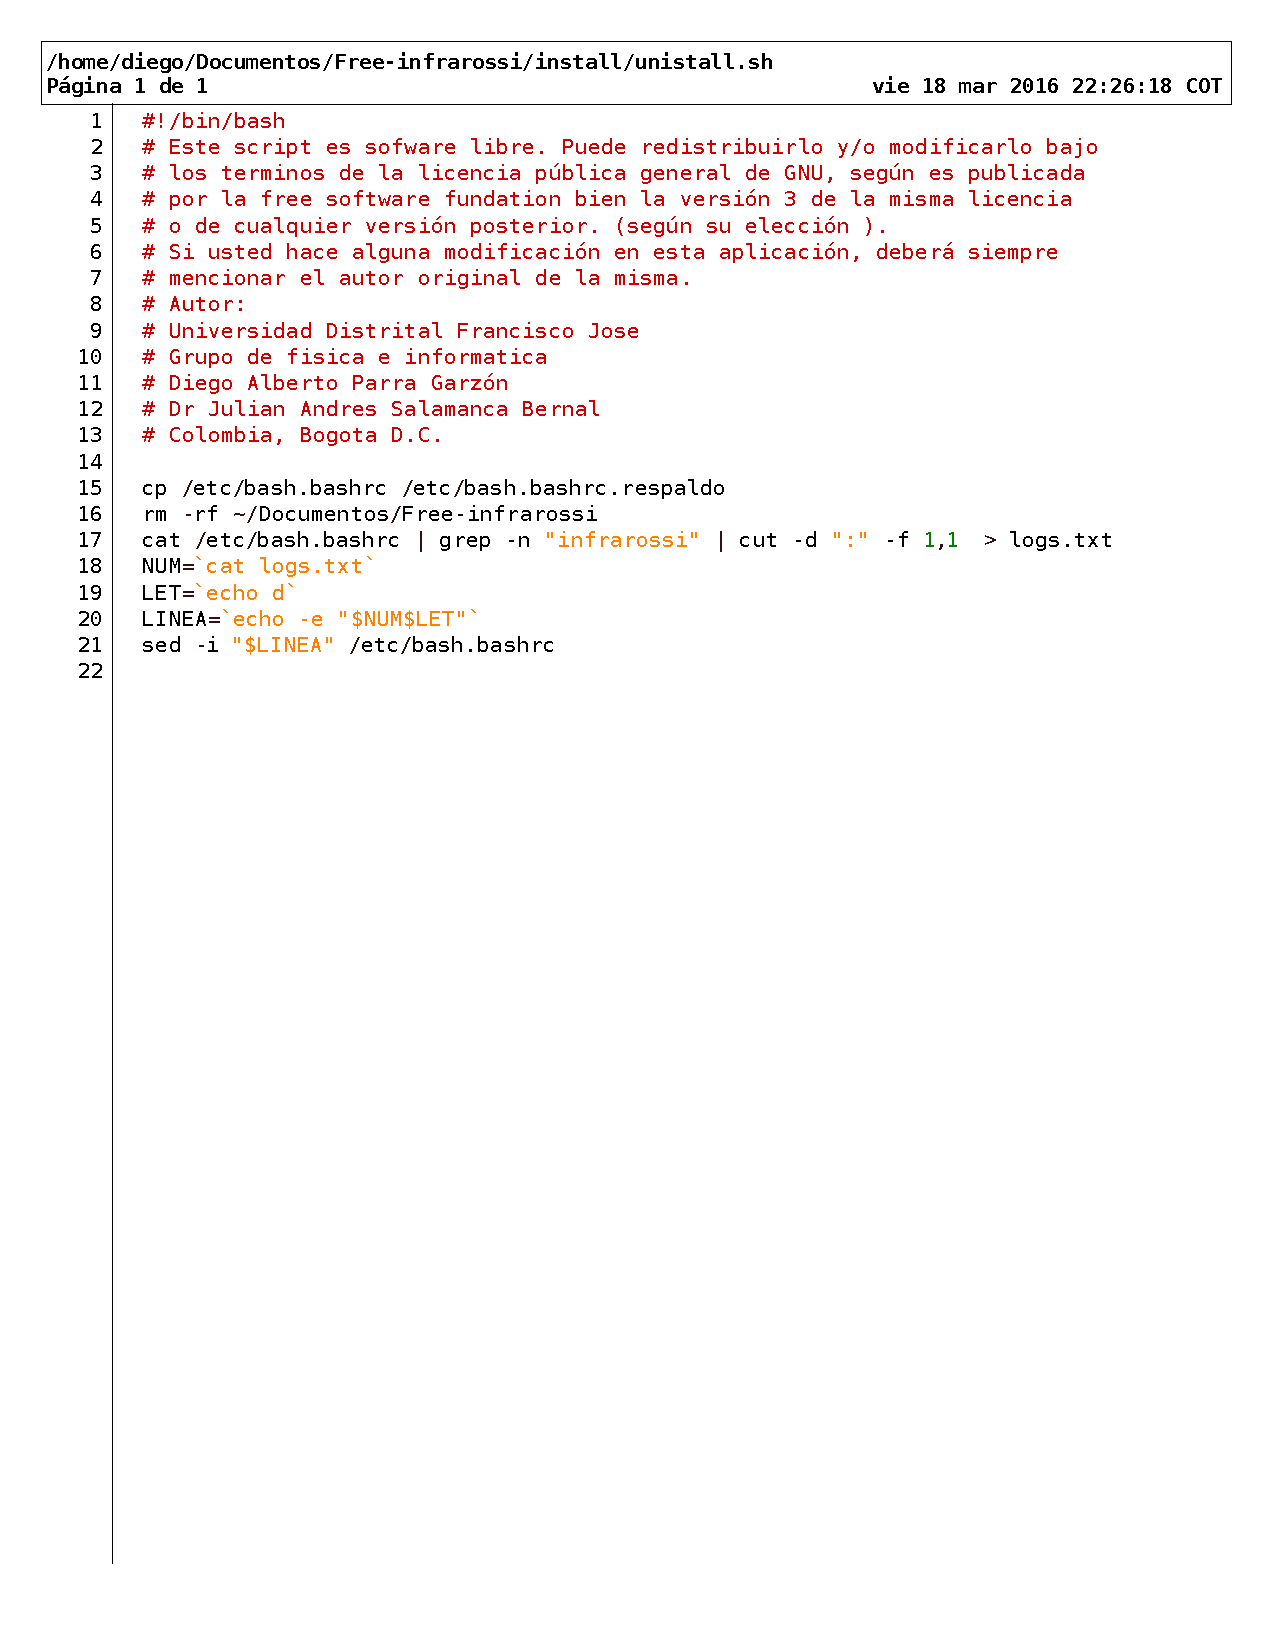
\includepdf[pages=-,scale=1,pagecommand={}]{unistall.pdf}
%----------------infrarossi.py
\subsection{infrarossi.py} \label{infrarossi}
Este código comienza en la pagina que sigue.
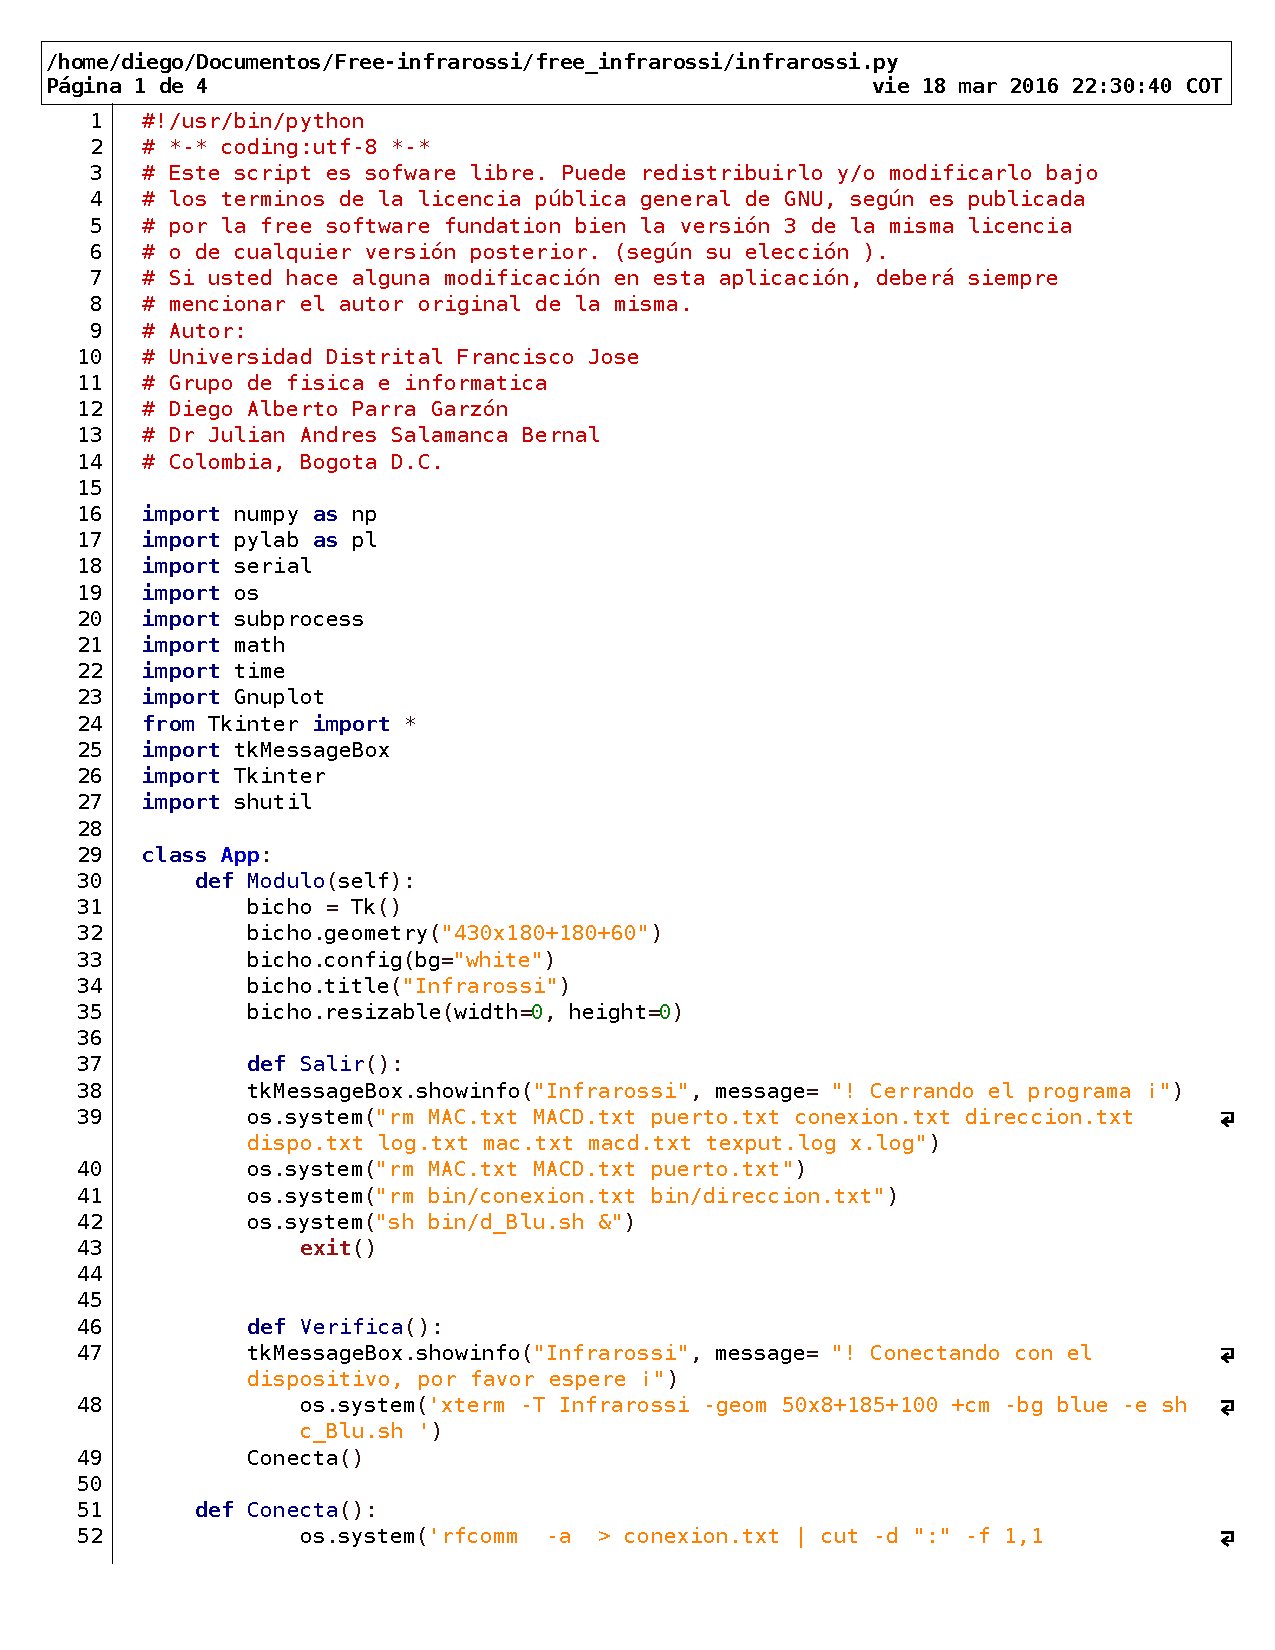
\includepdf[pages=-,scale=1,pagecommand={}]{infrarossi.pdf}  
%----------------infrarossi
\subsection{infrarossi}
Este código comienza en la pagina que sigue.
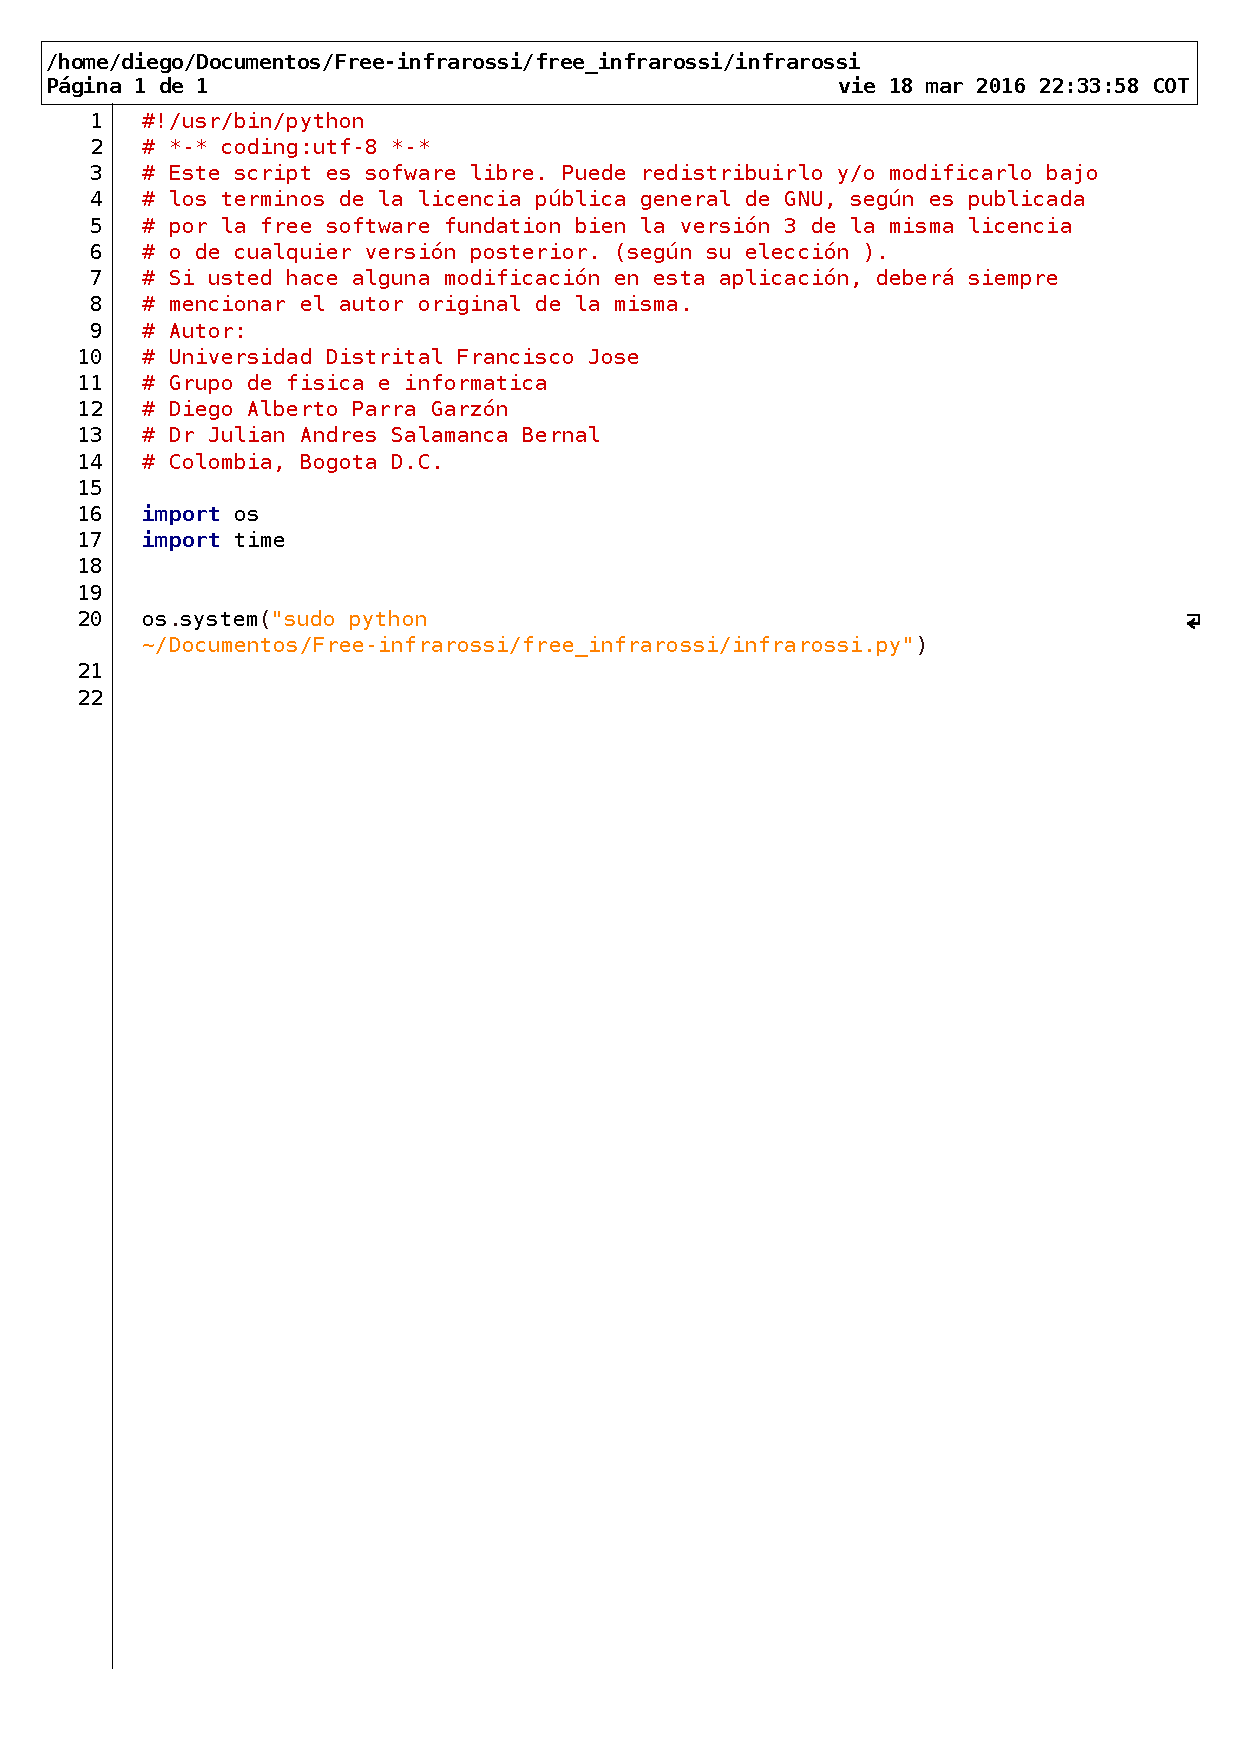
\includepdf[pages=-,scale=1,pagecommand={}]{infrarosssi.pdf}
%----------------c_Blue.sh
\subsection{c\_Blue.sh}
Este código comienza en la pagina que sigue.
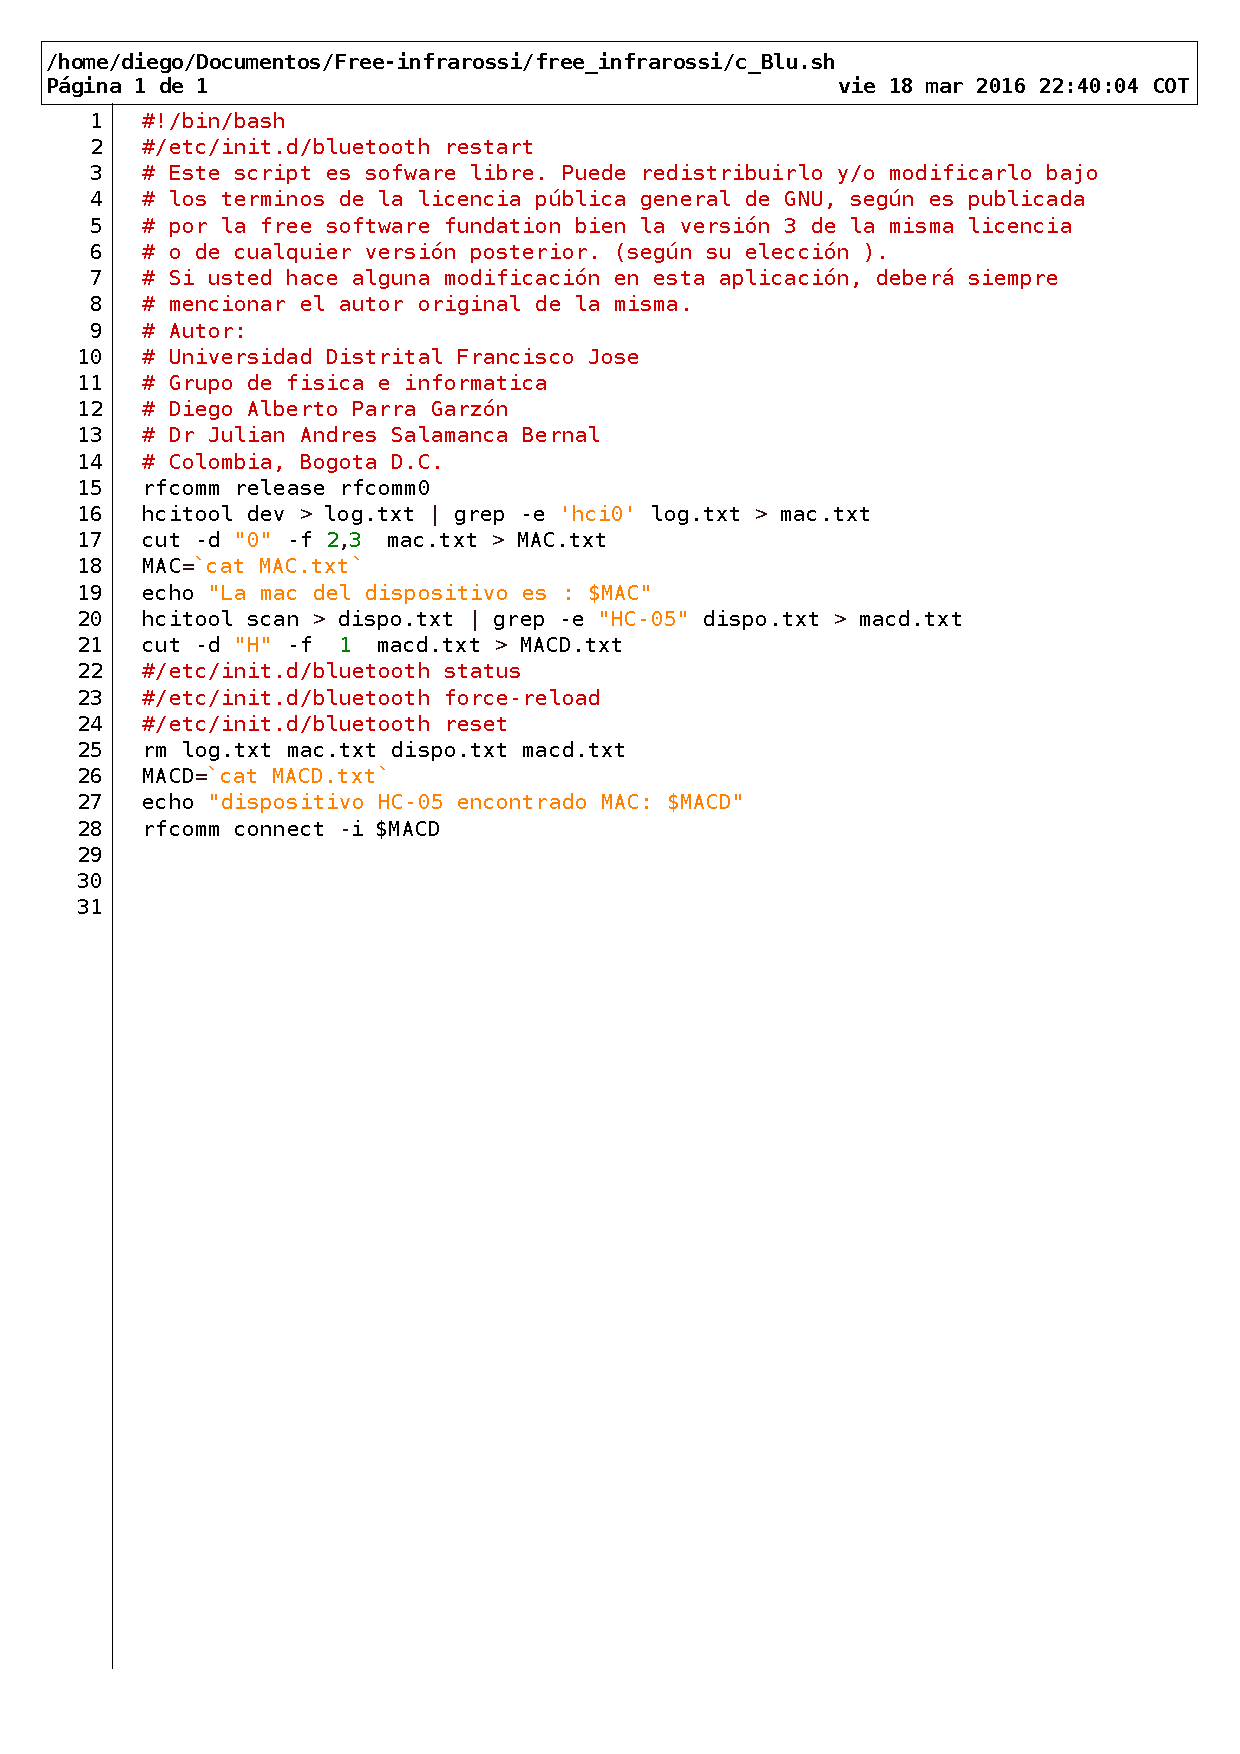
\includepdf[pages=-,scale=1,pagecommand={}]{cBlu.pdf}  
%----------------g_p_Abs.py
\subsection{g\_p\_Abs.py}
Este código comienza en la pagina que sigue.
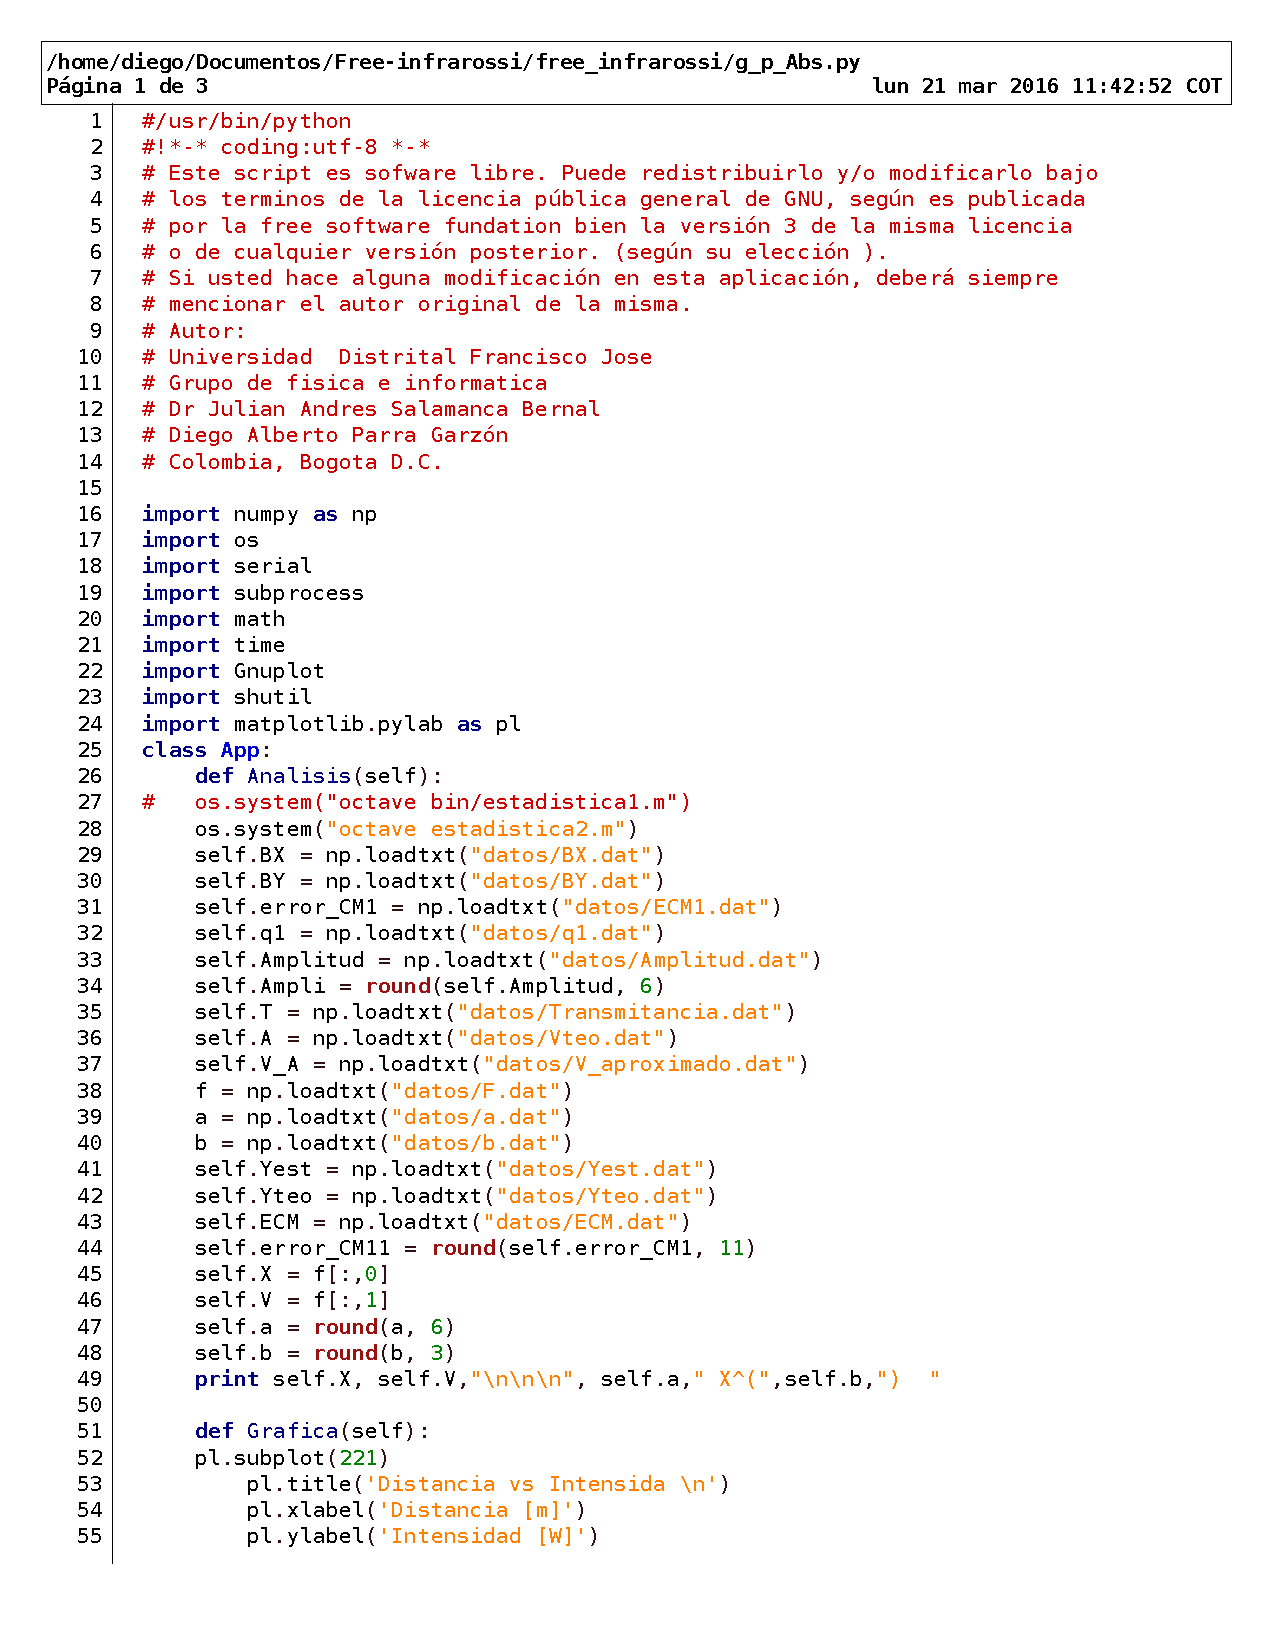
\includepdf[pages=-,scale=1,pagecommand={}]{gpAbs.pdf}    
%----------------g_p_Ate.py
\subsection{g\_p\_Ate.py}
Este código comienza en la pagina que sigue.
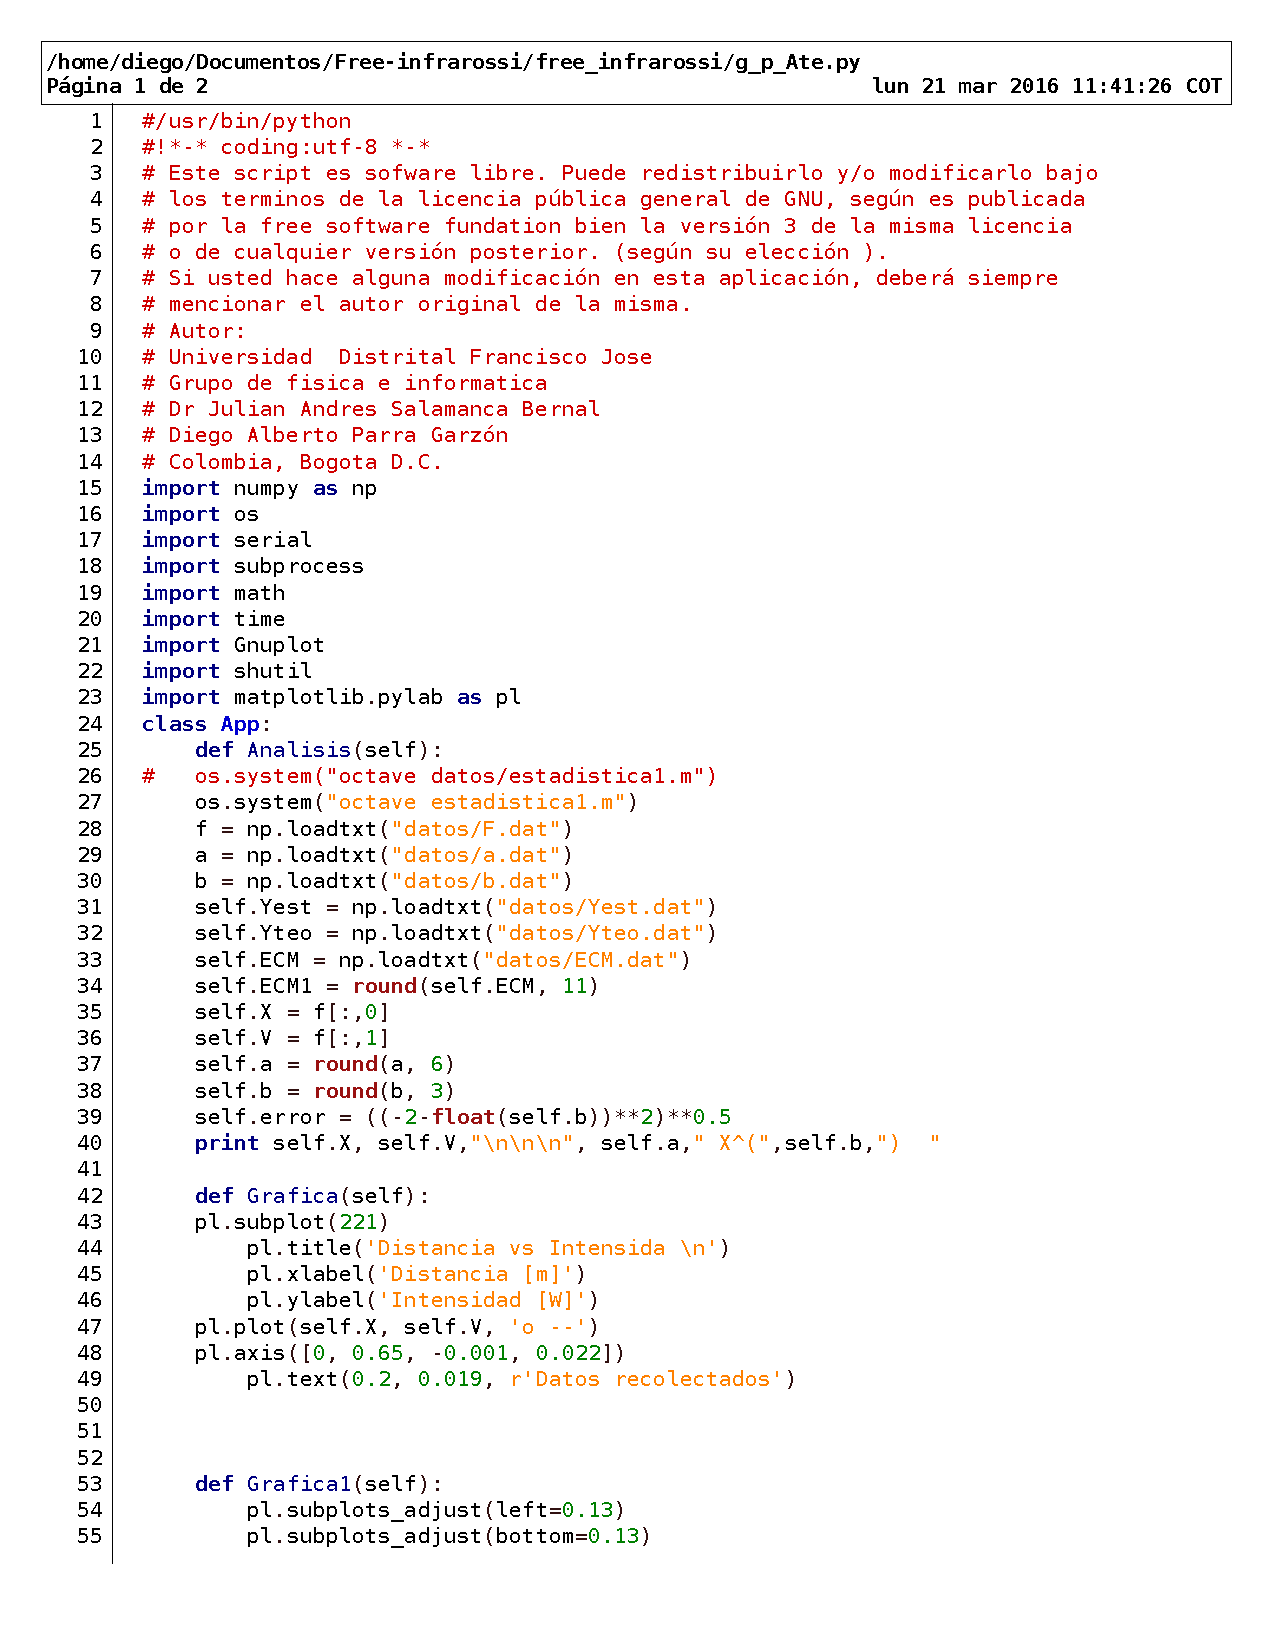
\includepdf[pages=-,scale=1,pagecommand={}]{gpAte.pdf} 
%----------------Estadistica1.m
\subsection{Estadistica1.m}
Este código comienza en la pagina que sigue.
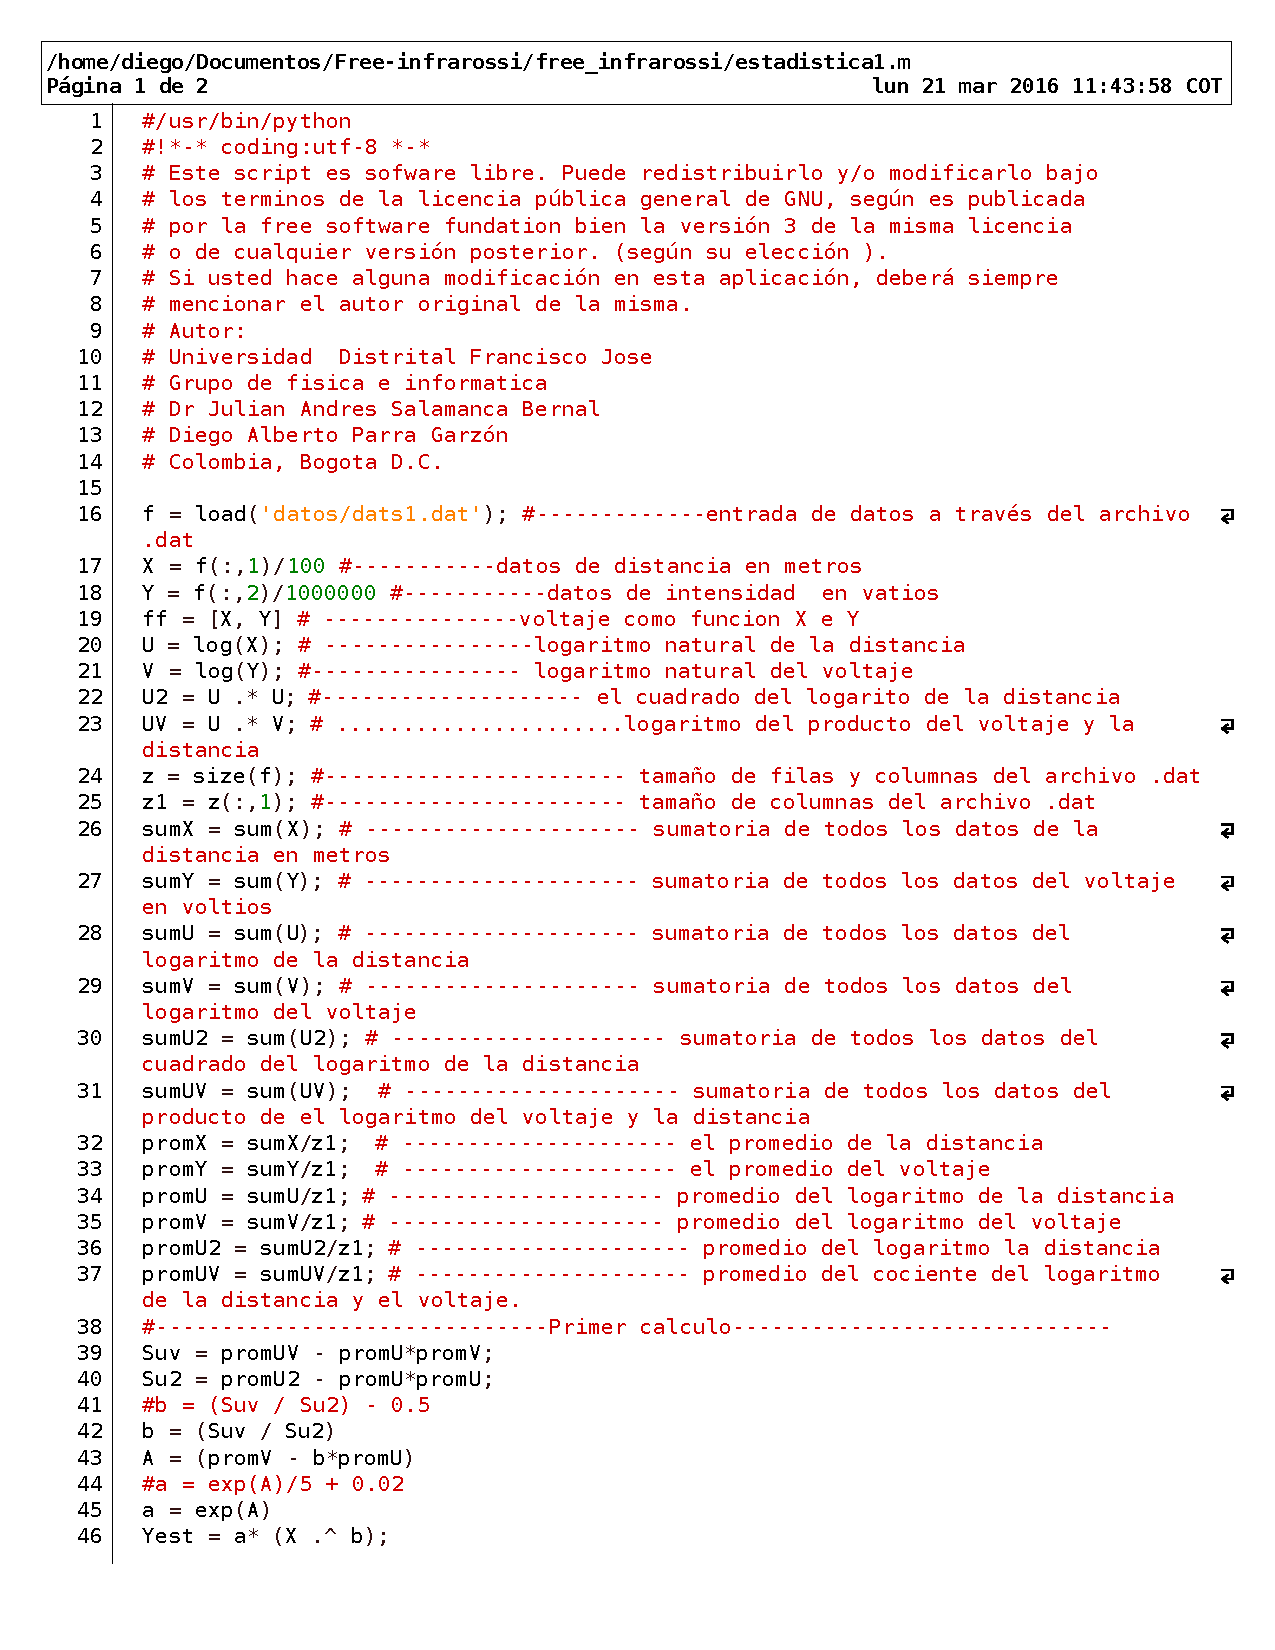
\includepdf[pages=-,scale=1,pagecommand={}]{estadistica1m.pdf} 
%----------------Estadistica2.m
\subsection{Estadistica2.m}
Este código comienza en la pagina que sigue.
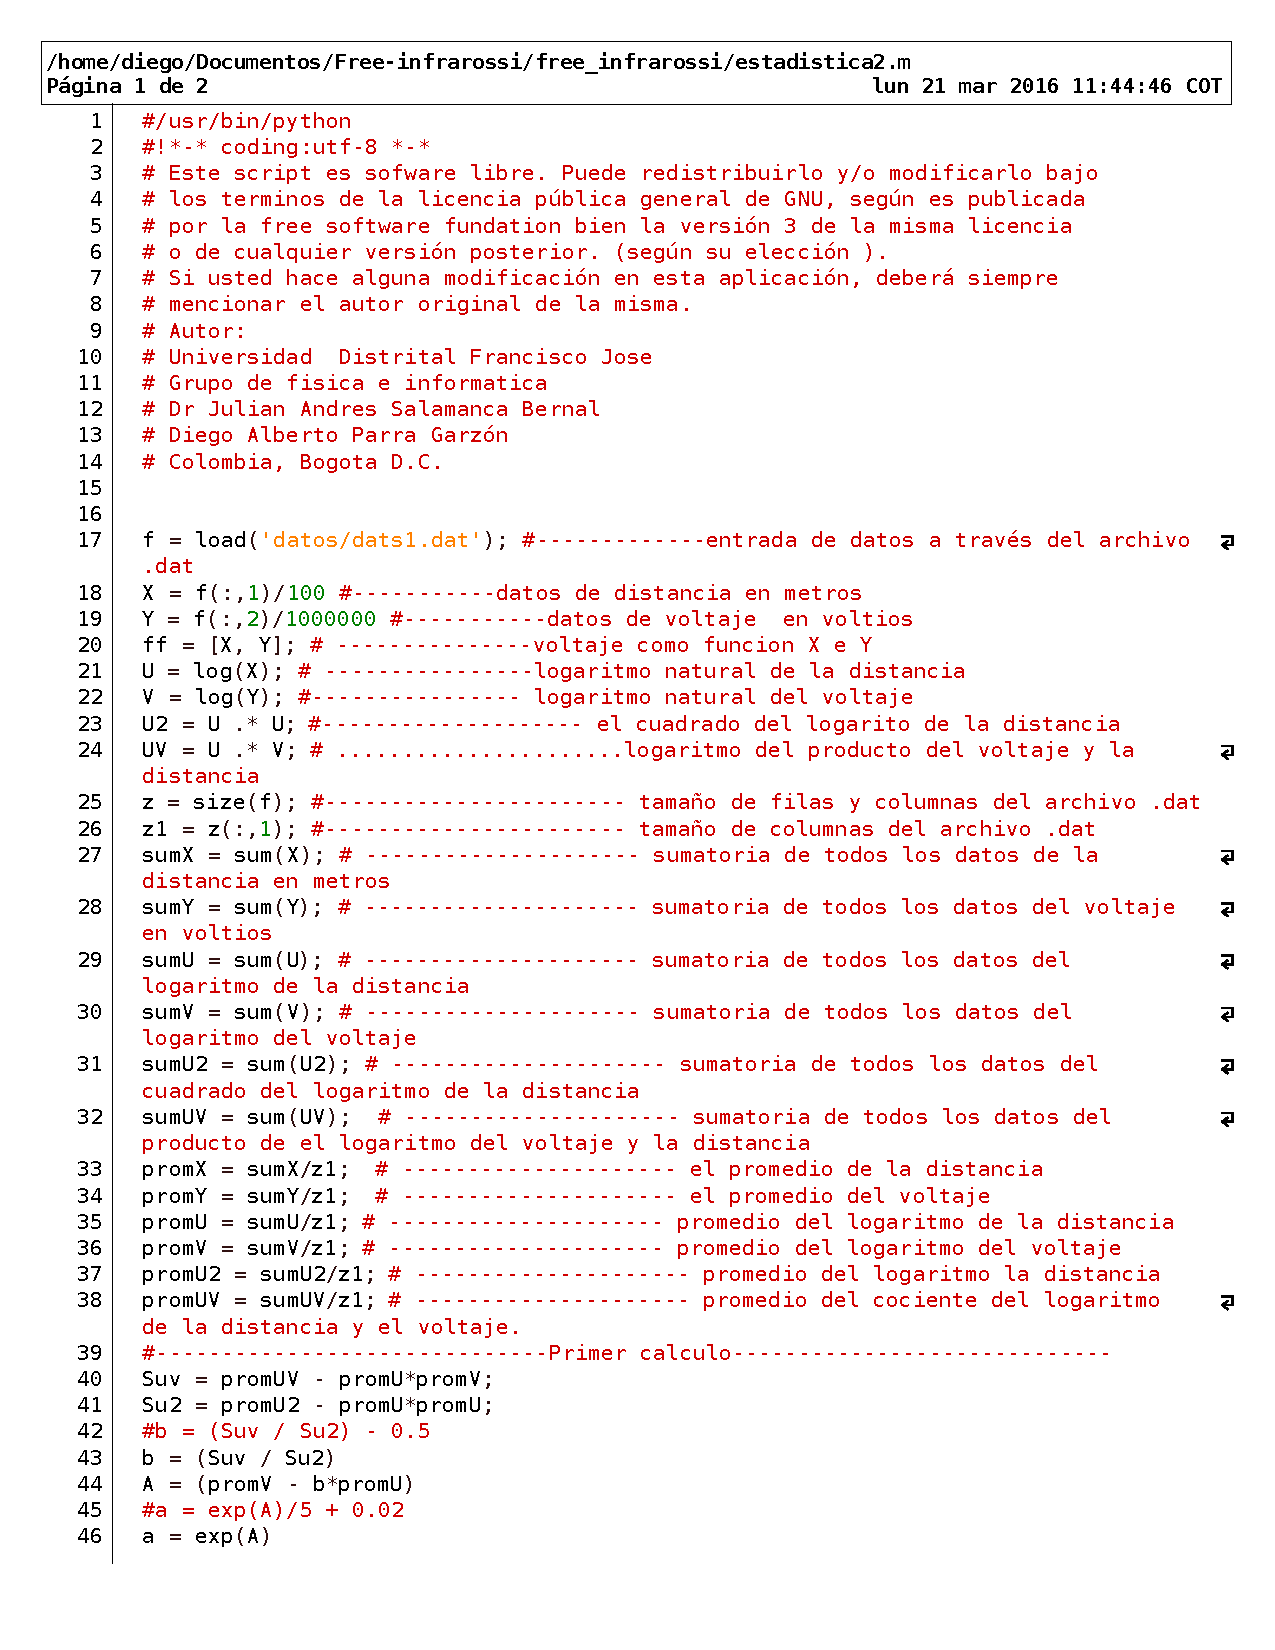
\includepdf[pages=-,scale=1,pagecommand={}]{estadistica2m.pdf}
%----------------Atenuacion.py
\subsection{Atenuacion.py}
Este código comienza en la pagina que sigue.
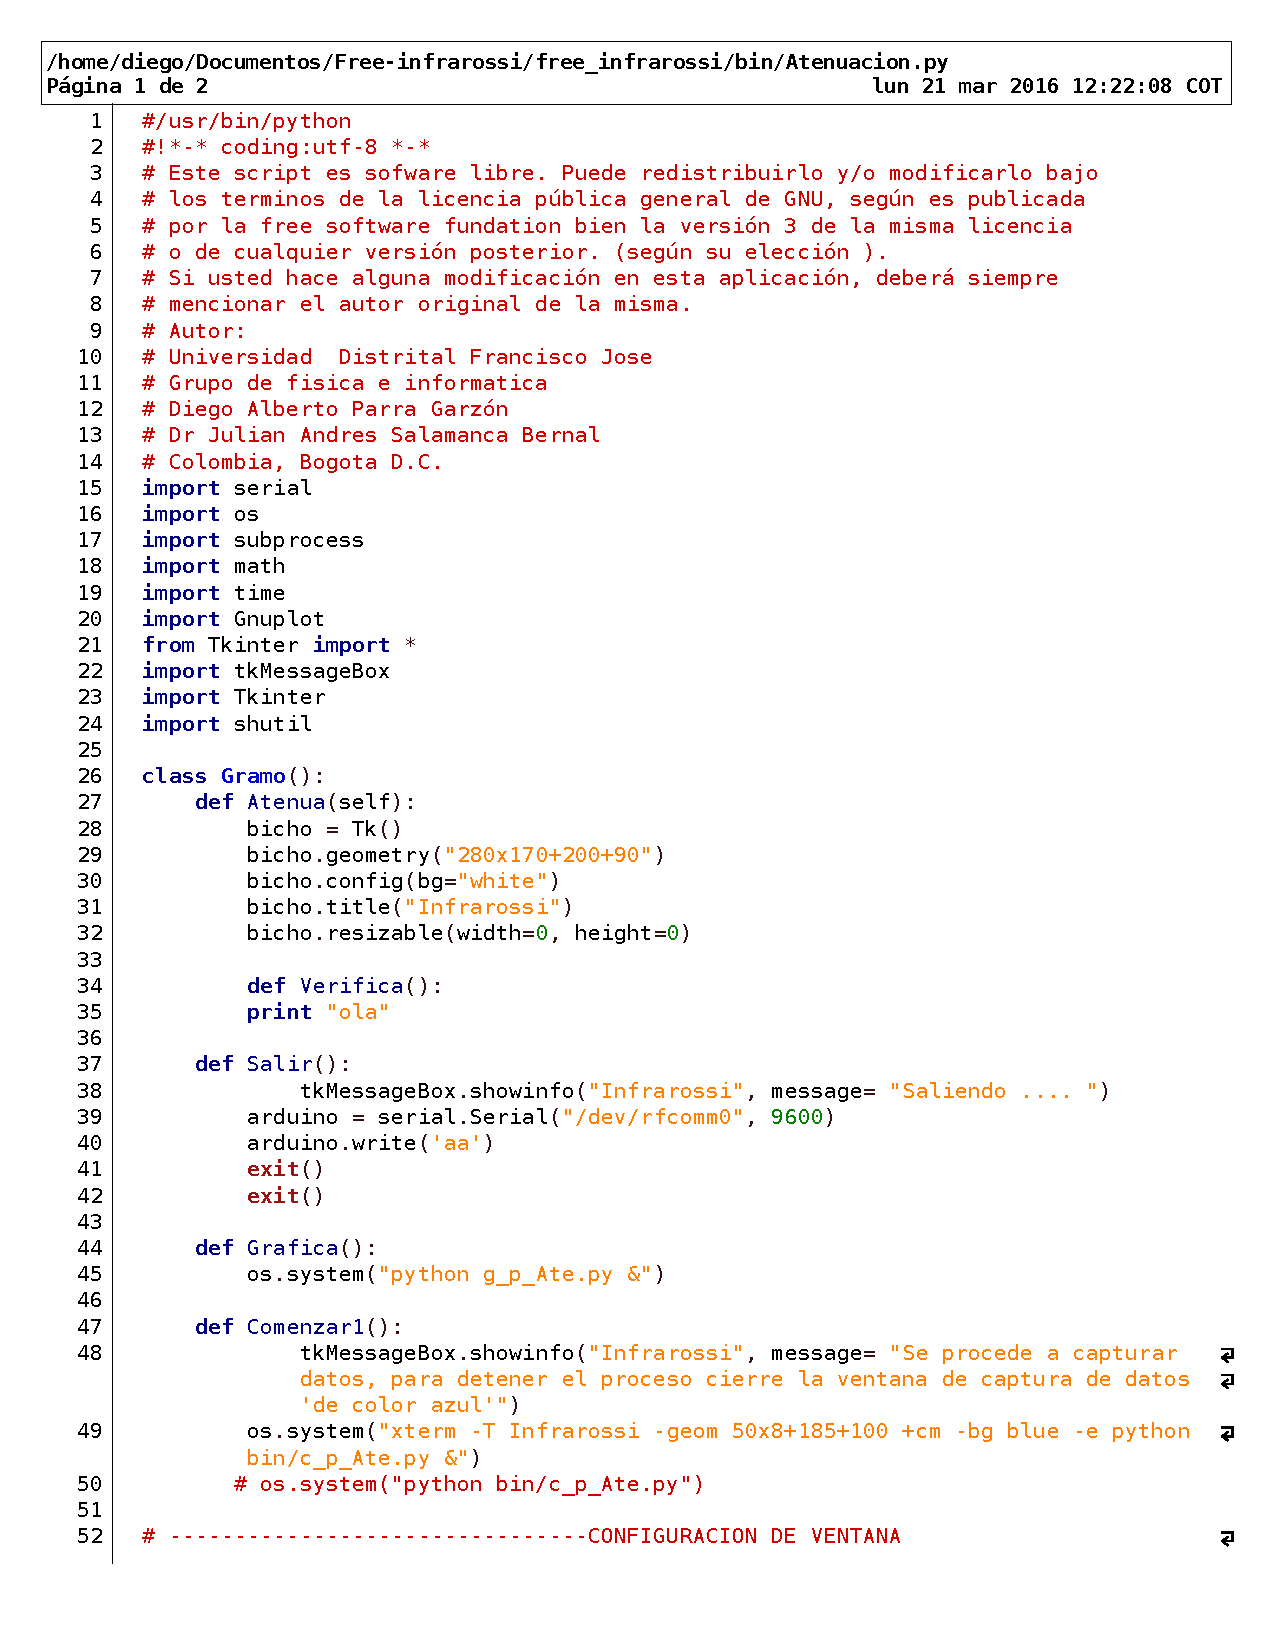
\includepdf[pages=-,scale=1,pagecommand={}]{Atenuacion.pdf}    
%----------------Absorcion.py
\subsection{Absorcion.py}
Este código comienza en la pagina que sigue.
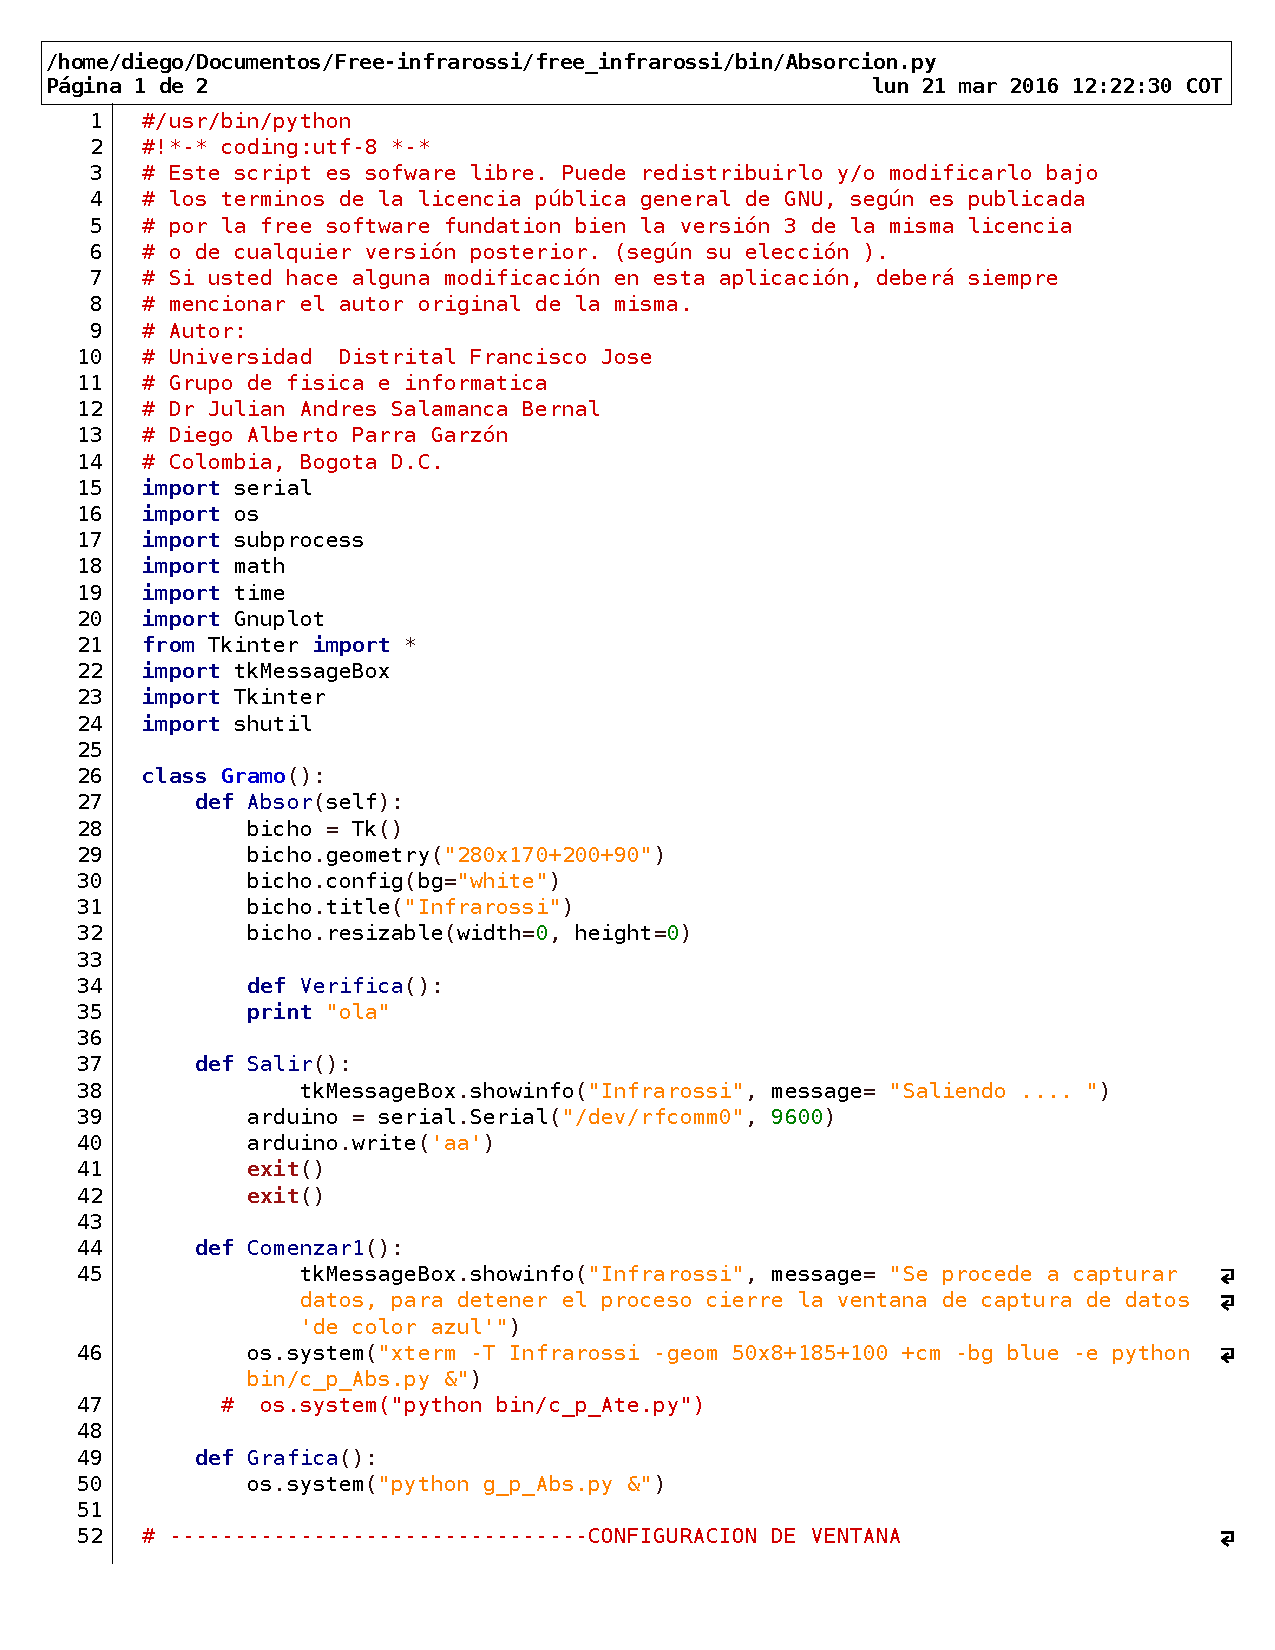
\includepdf[pages=-,scale=1,pagecommand={}]{Absorcion.pdf} 
%----------------Difraccion.py
\subsection{Difraccion.py}
Este código comienza en la pagina que sigue.
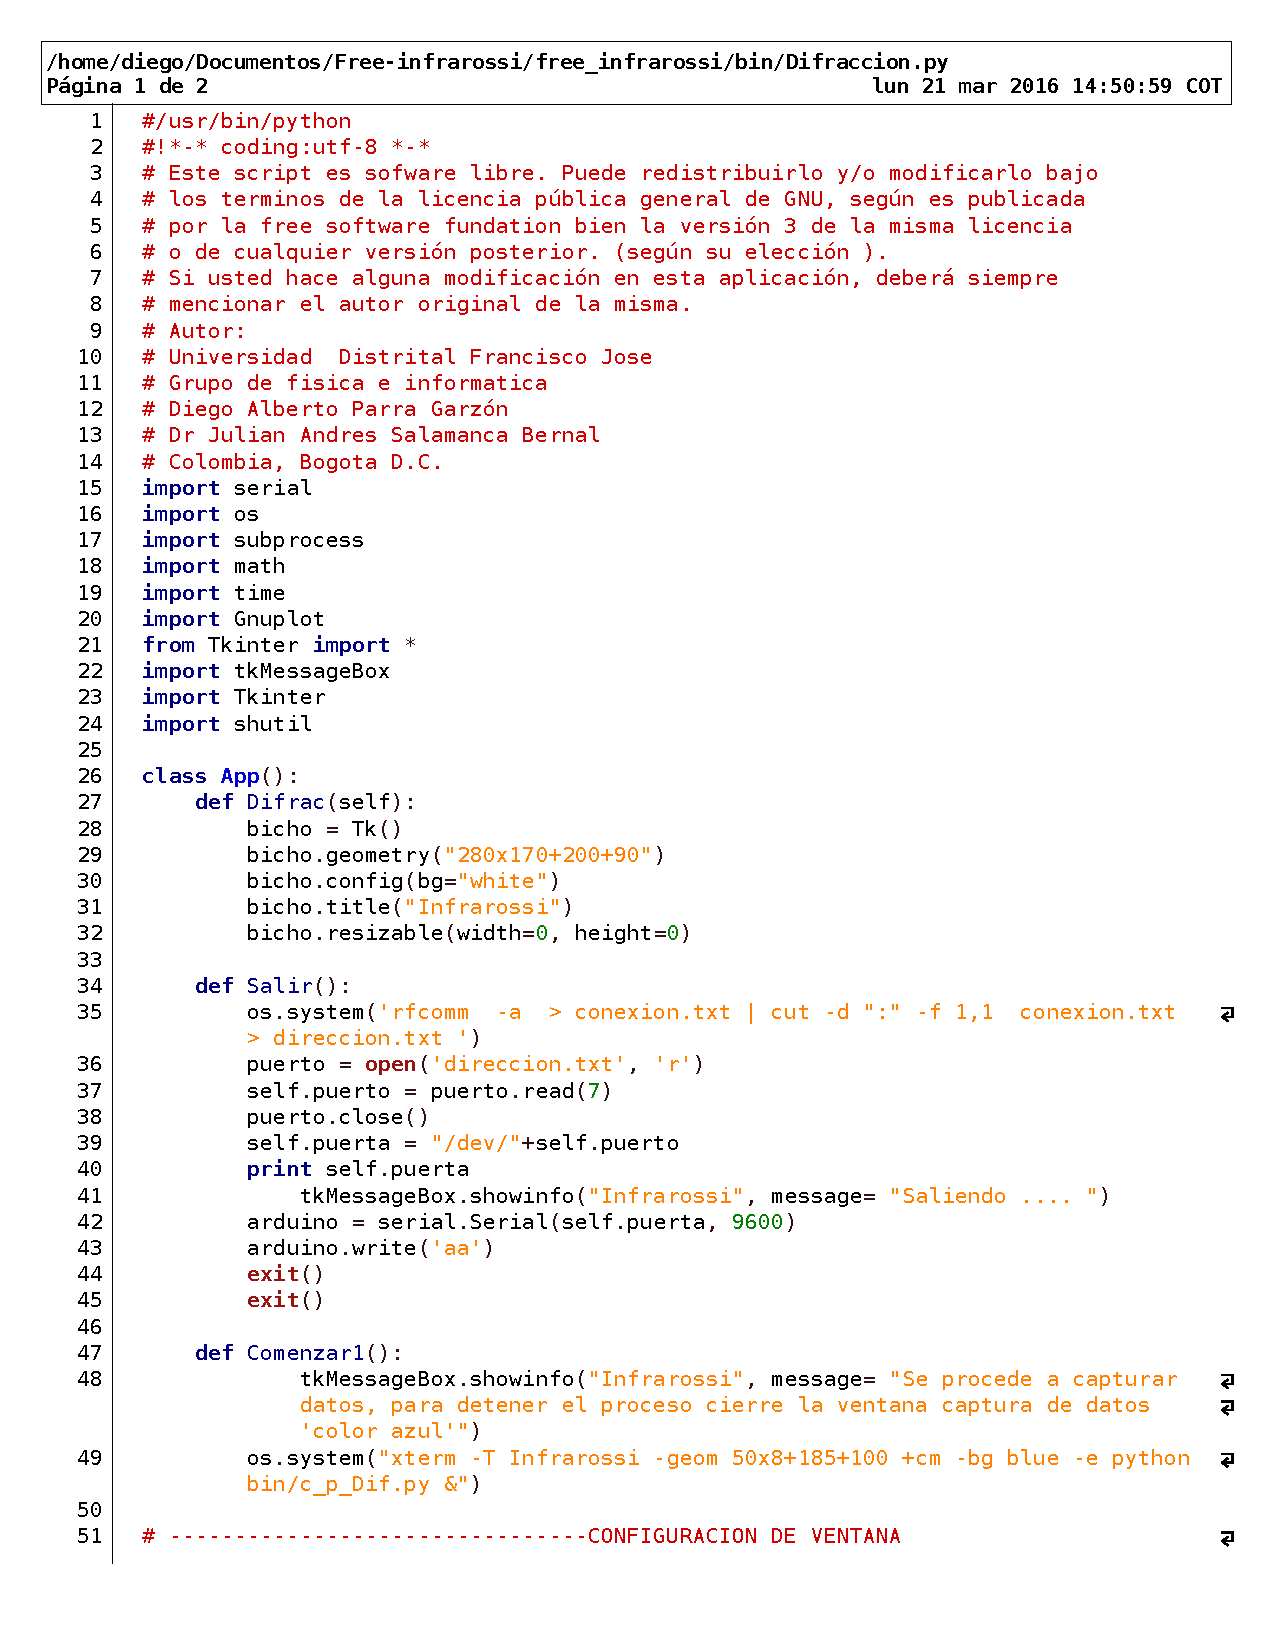
\includepdf[pages=-,scale=1,pagecommand={}]{Difraccionpy.pdf} 
%----------------c_p_Abs.py
\subsection{c\_p\_Abs.py}
Este código comienza en la pagina que sigue.
\includepdf[pages=-,scale=1,pagecommand={}]{cpAbs.pdf}    
%----------------c_p_Dif.py
\subsection{c\_p\_Dif.py}
Este código comienza en la pagina que sigue.
\includepdf[pages=-,scale=1,pagecommand={}]{cpDif.pdf} 
%----------------c_p_Ate.py
\subsection{c\_p\_Ate.py}
Este código comienza en la pagina que sigue.
\includepdf[pages=-,scale=1,pagecommand={}]{cpAte.pdf} 
%----------------Estadis2.py
\subsection{Estadis2.py}
Este código comienza en la pagina que sigue.
\includepdf[pages=-,scale=1,pagecommand={}]{estadis2py.pdf} 
%----------------o_Carpestas.py
\subsection{o\_Carpetas.py}
Este código comienza en la pagina que sigue.
\includepdf[pages=-,scale=1,pagecommand={}]{oCarpetaspy.pdf}
%----------------o_Carpestas1.py
\subsection{o\_Carpetas1.py}
Este código comienza en la pagina que sigue.
\includepdf[pages=-,scale=1,pagecommand={}]{oCarpetas1.pdf} 
%----------------o_Carpestas2.py
\subsection{o\_Carpetas2.py}
Este código comienza en la pagina que sigue.
\includepdf[pages=-,scale=1,pagecommand={}]{oCarpeta2.pdf} 
%----------------o_Carpeta.sh
\subsection{m\_Carpeta.sh}
Este código comienza en la pagina que sigue.
\includepdf[pages=-,scale=1,pagecommand={}]{mCarpetash.pdf} 
%----------------m_Carpestas1.sh
\subsection{m\_Carpetas1.sh}
Este código comienza en la pagina que sigue.
\includepdf[pages=-,scale=1,pagecommand={}]{mCarpeta1sh.pdf} 
%----------------o_Carpestas2.sh
\subsection{m\_Carpetas2.sh}
Este código comienza en la pagina que sigue.
\includepdf[pages=-,scale=1,pagecommand={}]{mCarpeta2sh.pdf} 

%----------------G_firmware.py
\subsection{G\_firmware.py}
Este código comienza en la pagina que sigue.
\includepdf[pages=-,scale=1,pagecommand={}]{Gfirmawarepy.pdf}  
%----------------firmwarefreeinfrarossi.py
\subsection{firmware\_free\_infrarossi.py}
Este código comienza en la pagina que sigue.
\includepdf[pages=-,scale=1,pagecommand={}]{firmwarefreeinfrarossipy.pdf} 
%----------------infrarossi.cpp
\subsection{infrarossi.cpp}
Este código comienza en la pagina que sigue.
\includepdf[pages=-,scale=1,pagecommand={}]{infrarossicpp.pdf} 
%----------------infrarossi.hex
\subsection{infrarossi.hex}
Este código comienza en la pagina que sigue.
\includepdf[pages=-,scale=1,pagecommand={}]{infrarossihex.pdf} 

\end{document}
